%% BioMed_Central_Tex_Template_v1.06    %
%%                                      %

% Multi-subject/DLA EMG-based control of mechanical hands
% Castellini, Fiorilla, Sandini
%
% Submitted to J NeuroEng Rehab, December, 2008
% Resubmitted w/ new reviewers, March, 2009
% Accepted under revision, June, 2009

\NeedsTeXFormat{LaTeX2e}[1995/12/01]
\documentclass[10pt]{bmc_article}    

\usepackage{cite} % Make references as [1-4], not [1,2,3,4]
\usepackage{url}  % Formatting web addresses  
\usepackage{ifthen}  % Conditional 
\usepackage{multicol}   %Columns
%\usepackage[utf8]{inputenc} %unicode support
\usepackage{amsmath}
\usepackage[psamsfonts]{amssymb}
\urlstyle{rm}
 
\def\includegraphic{}
\def\includegraphics{}

\setlength{\topmargin}{0.0cm}
\setlength{\textheight}{21.5cm}
\setlength{\oddsidemargin}{0cm} 
\setlength{\textwidth}{16.5cm}
\setlength{\columnsep}{0.6cm}

\newboolean{publ}

%Review style settings
\newenvironment{bmcformat}{\begin{raggedright}\baselineskip20pt\sloppy\setboolean{publ}{false}}{\end{raggedright}\baselineskip20pt\sloppy}
%Publication style settings
%\newenvironment{bmcformat}{\fussy\setboolean{publ}{true}}{\fussy}

\def\RR{\mathbb{R}}
\def\NN{\mathbb{N}}
\def\xx{\mathbf{x}}
\def\yy{\mathbf{y}}
\def\ww{\mathbf{w}}

\begin{document}

\begin{bmcformat}

\title{Multi-subject / Daily-Life Activity\\EMG-based control of mechanical hands}
 
\author{%
  Claudio Castellini\correspondingauthor$^1$%
  \email{Claudio Castellini - claudio.castellini@unige.it}%
\and
  Angelo Emanuele Fiorilla$^{2,3}$%
  \email{Angelo Emanuele Fiorilla - emanuele.fiorilla@iit.it}%
\and
  Giulio Sandini$^3$%
  \email{Giulio Sandini - giulio.sandini@iit.it}%
}%

\address{%
    \iid(1)LIRA-Lab, University of Genova, viale F. Causa 13, 16145 Genova, Italy\\
    \iid(2)DIST, University of Genova, viale F. Causa 13, 16145 Genova, Italy\\
    \iid(3)Italian Institute of Technology, via Morego 30, 16163 Genova, Italy
}%

\maketitle

\begin{abstract}

\paragraph*{Background:}

forearm surface electromyography (EMG) has been in use since the Sixties
to feed-forward control active hand prostheses in a more and more refined way.
Recent research shows that it can be used to control even a dexterous
polyarticulate hand prosthesis such as Touch Bionics's i-LIMB,
as well as a multifingered, multi-degree-of-freedom mechanical hand such
as the DLR II. In this paper we extend previous work and investigate
the robustness of such fine control possibilities, in two ways: firstly,
we conduct an analysis on data obtained from $10$ healthy subjects, trying
to assess the general applicability of the technique; secondly, we compare
the baseline controlled condition (arm relaxed and still on a table) with
a ``Daily-Life Activity'' condition in which subjects walk, raise
their hands and arms, sit down and stand up, etc., as an experimental proxy
of what a patient is supposed to do in real life.
We also propose a cross-subject model analysis,
i.e., training a model on a subject and testing it on another one. The use
of pre-trained models could be useful in shortening the time required by
the subject / patient to become proficient in using the hand.

\paragraph*{Results:}

a standard machine learning technique was able to achieve a real-time grip
posture classification rate of about $97\%$ in the baseline condition and
$95\%$ in the DLA condition; and an average correlation ot the target of
about $0.93$ ($0.90$) while reconstructing the required force. Cross-subject analysis
is encouraging although not definitive in its present state.

\paragraph*{Conclusions:}

performance figures obtained here are in the same order of magnitude of
those obtained in previous work about healthy subjects in controlled conditions
and/or amputees, which lets us claim that this technique can be used
by reasonably any subject, and in DLA situations. Use of previously trained
models is not fully assessed here, but more recent work indicates it is a
promising way ahead.

\end{abstract}

\ifthenelse{\boolean{publ}}{\begin{multicols}{2}}{}

\section*{Background}
\label{sec:introduction}

Electromyography (EMG from now on) is a well-known diagnostic tool
for detecting muscle disorders from motor unit activation potentials
\cite{deluca97,deluca02}. In its non-invasive (surface) version it
has also been used since the Sixties \cite{bottomley65,childress69,sears}
to enable amputees control one or two degrees-of-freedom (DOFs)
of active upper limb prostheses. Its commercial / clinical applications
include, e.g., Otto Bock's SensorHand Speed \cite{sensorhand}, the Motion
Control Hand and the Utah Arm \cite{mchand}, and more recently,
Touch Bionics's i-LIMB \cite{ilimb}, with $5$ active and one passive DOF.
In some of these cases, force / torque are also controlled.

The popularity of surface EMG stems from its cheapness, simplicity of use
and non-invasiveness. Nevertheless, research on more and more dexterous
mechanical hands is ongoing (e.g., the DLR-II hand \cite{Hua2006} and the
Cyberhand \cite{cyberhand,cipriani}) and soon a finer control will be
required. To this end, at least since 2002
\cite{dunlop,zecca,smagt,2008.ICRA} it is known that a few surface EMG
electrodes suffice to recognise up to nine isometric/isotonic hand postures.
This potentiality has so far been exploited clinically in the i-LIMB only,
and to a very limited extent so far, as far as we know. In previous work
it has also been shown that a dexterous hand prosthesis can be
feed-forward force-controlled \emph{while} detecting
grasping postures \cite{2008.ICRA,2008.BioCyb} in real time.
So it appears that plain, old EMG still has to be exploited in full.

The work presented in this paper fits in this line of research,
extending previous results along two ``orthogonal'' directions: first, we analyse
data collected from $10$ healthy subjects and thus try and assess the general
applicability of the technique; second, we compare a baseline controlled
condition with a ``Daily-Life Activity'' (DLA) one, in which subjects walk, raise
their hands and arms, sit down and stand up, etc., while performing the same
actions of the baseline. The DLA condition is an experimental proxy
of what a patient is supposed to do in real life. Lastly, we propose a
cross-subject model analysis, i.e., training a
model on a subject and testing it on another one. The use
of pre-trained models could be useful in shortening the time required by
the subject / patient to become proficient in using the prosthesis.

\section*{Materials and Methods}
\label{sec:m&ms}

\subsection*{Subjects}

Ten healthy subjects joined the experiment after having given their informed
consent. The subjects were two women and eight men, nine right-handed and one
left-handed, average age $30.9 \pm 8.45$ years, standard Caucasian weight and
height. They were given no knowledge of what the experiment was about.

\subsection*{Experimental procedure}

The experiment consisted of two phases.
During phase $1$, after a ``rest'' condition was sampled to define the baseline
EMG activity, the subject would keep her/his arm still and relaxed
on a table, and was asked to grasp a force sensor using, in turn,
three different ways of grasping it (Figure \ref{fig:Grasps}):
index precision grip, other fingers precision grip and power grasp.
While gathering data, a label $\{1,2,3,4\}$ denoting the grasp (or rest)
was attached to each sample, in order to build the ground truth values.

%\begin{figure*}[!t] \centering
%  \begin{tabular}{ccc}
%    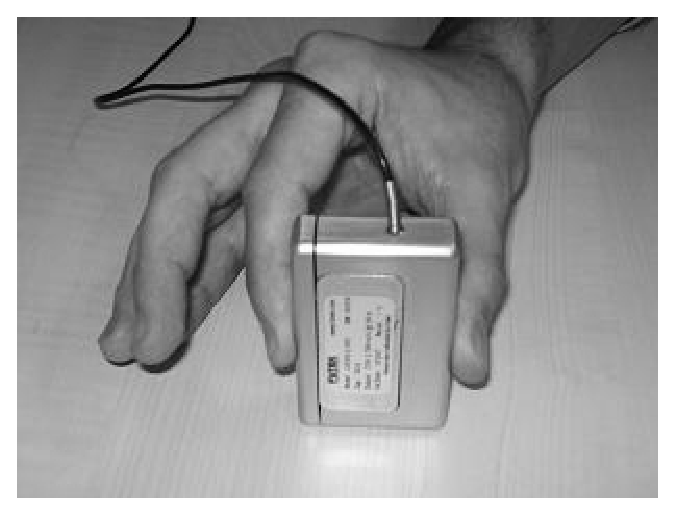
\includegraphics[height=0.16\textheight]{grip1.eps} &
%    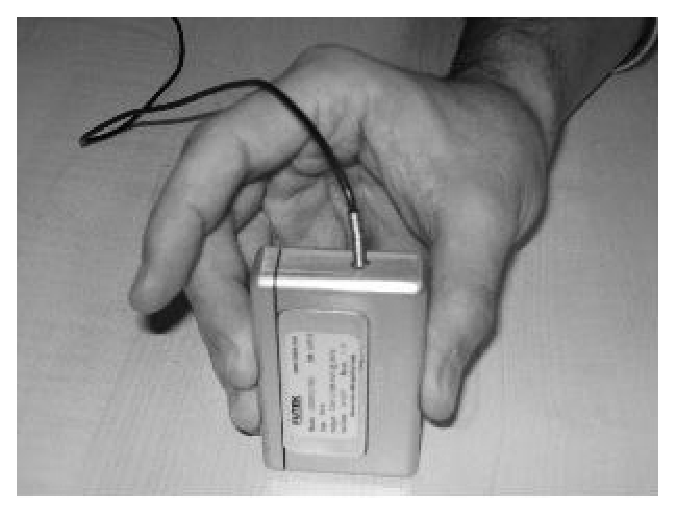
\includegraphics[height=0.16\textheight]{grip2.eps} &
%    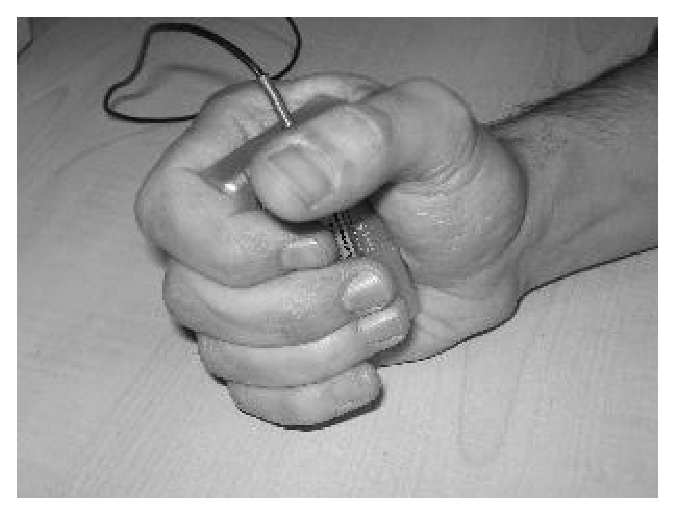
\includegraphics[height=0.16\textheight]{grip3.eps} \\
%    $(a)$ & $(b)$ & $(c)$ \\
%  \end{tabular}
%  \caption{The three different grips employed in the experiment: $(a)$
%   index precision grip; $(b)$ other fingers precision grip; $(c)$
%   power grasp.}
%  \label{fig:Grasps}
%\end{figure*}

The subject freely repeated each grasping action for
$100$'', resting for $30$'' in between grasps. The whole procedure was
repeated twice for numerical robustness purposes. This ``baseline''
phase will be referred to from now on as the \emph{Still-Arm phase (SA)}.

Phase $2$, which started soon after phase $1$ for each subject,
consisted in repeating phase $1$ while the subject was left free to
move, walk around, lift and pronate / supinate the
arm and forearm, sit down and stand up from a chair. This 
second phase is intended as a laboratory-controlled proxy 
of the main movements a patient is expected to do during DLAs.
This phase will be called \emph{Free-Arm phase (FA)}.

Each subject's experiment resulted in something more than
$1200$'' of data. Data were sampled at $2$KHz, resulting in
about $2.4\times 10^6$ samples for each subject, equally
distributed in each phase.

\subsection*{Equipment and electrode placement}

%\begin{figure*}[!t] \centering
%  \begin{tabular}{ccc}
%    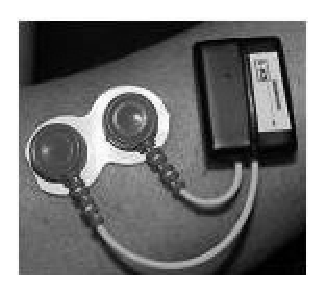
\includegraphics[height=0.16\textheight]{Electrode.eps} &
%    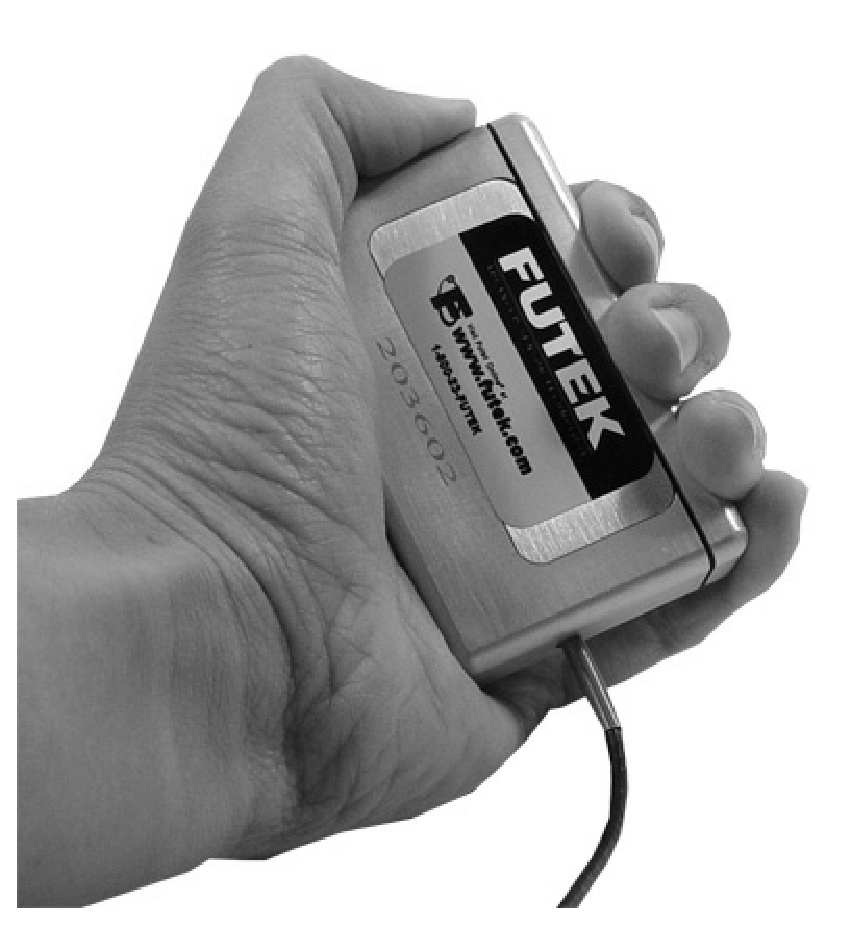
\includegraphics[height=0.16\textheight]{Hand_Gripper.eps} &
%    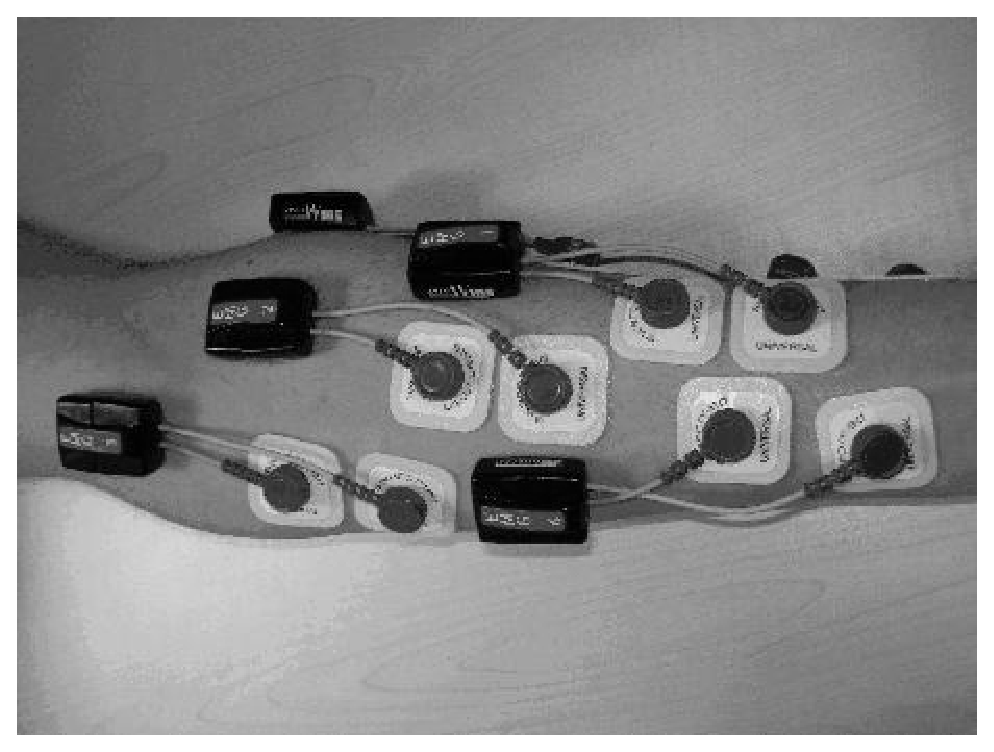
\includegraphics[height=0.16\textheight]{El_Arrangement.eps} \\
%    $(a)$ & $(b)$ & $(c)$ \\
%  \end{tabular}
%  \caption{The experimental setup (\textit{subject side}): $(a)$ an EMG
%    wireless electrode; $(b)$ the FUTEK force sensor; $(c)$ the typical
%    placement of the EMG electrodes on a subject's forearm (ventral side).}
%  \label{fig:SubjSetup}
%\end{figure*}

We employed Aurion ZeroWire wireless surface EMG
electrodes \cite{zerowire}, in order to ease the FA
phase, which required free movement in the laboratory. A FUTEK LMD500
Hand Gripper force sensor \cite{LMD500} was used to detect the
force applied while grasping. (See Figure \ref{fig:SubjSetup} $(a,b)$.)
A standard digital acquisition board
(National Instruments NI-USB6211) was used to record the signals,
connected to the receiver of the EMG wireless device and to an
amplifier, in turn connected to the force sensor. The sampling rate was set at
$2$KHz in order to correctly sample both signals\footnote{The EMG signal
relevant bandwidth lies between $15$ and $500$Hz.}. The board was connected via a
USB port to an entry-level laptop. We used a custom National
Instruments' LabView VI block to acquire the signals.

%\begin{figure*}[!t] \centering
%  \begin{tabular}{cc}
%    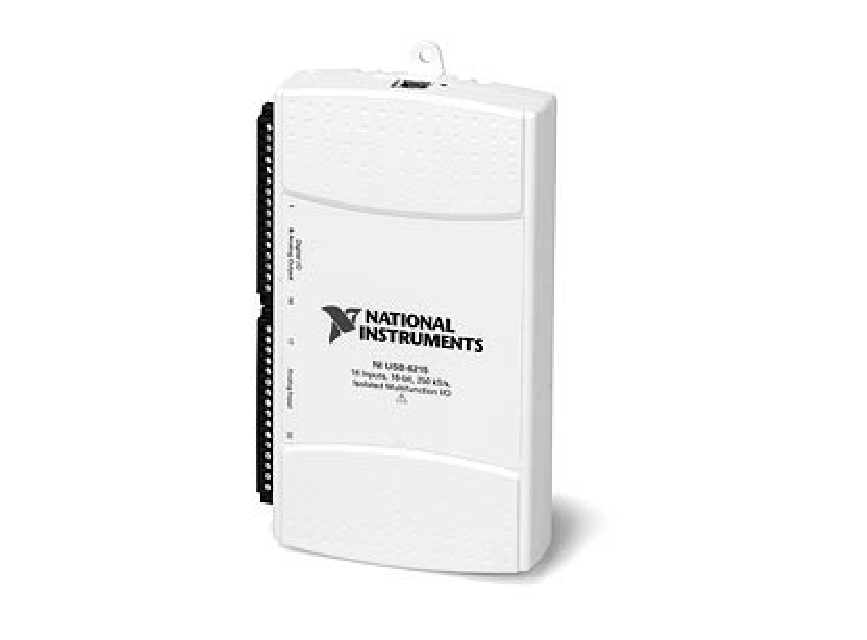
\includegraphics[height=0.16\textheight]{NI-6211.eps} &
%    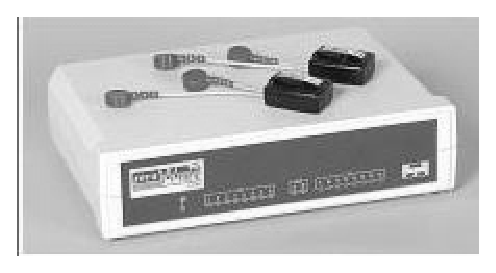
\includegraphics[height=0.16\textheight]{Zero_Base.eps} \\
%  $(a)$ & $(b)$\\
%  \end{tabular}
%  \caption{The experimental setup (\textit{experimenter side}): $(a)$
%   the USB data acquisition card (NI-USB6211); $(b)$ the EMG device
%   receiver.}
%  \label{fig:ExpSetup}
%\end{figure*}

Seven electrodes were glued on each subject's dominant
forearm, according to this anatomic guideline:

\begin{itemize}

  \item on the forearm ventral side: near the wrist, above the
    \emph{flexor pollicis longus}; centrally, above the \emph{flexor
    digitorum superficialis}; near the elbow, above the \emph{flexor
    digitorum profundus}; and near the wrist, above the \emph{flexor
    digitorum superficialis} again;

  \item on the forearm dorsal side: near the wrist, above the
    \emph{extensor pollicis brevis / abductor pollicis longus};
    centrally, above the \emph{extensor digitorum communis} and
    \emph{extensor digiti minimi}.

\end{itemize}

These positions were chosen, according to the medical \cite{Kendall} and
bioengineering \cite{kampas} literature, to detect the activity of the flexor
and extensor muscles of the forearm which are most relevant during grasping.
Figure \ref{fig:SubjSetup} $(c)$ shows
the typical electrode positioning. Notice that there may be remarkable
inter-arm differences depending on the subjects' age, gender and physical
fitness. Moreover, some of the aforementioned muscles are deep into
the forearm, so that muscle cross-talk cannot be avoided. This is a
well-known problem in the EMG literature \cite{deluca97,zecca}.

\subsection*{Data analysis}

The root-mean-square (RMS) of the EMG was evaluated using a time window
$T_{RMS}$\footnote{The choice of the RMS, as opposed
to the simpler rectification and filtering,
is motivated by its well-known relationship to the force exerted
by the related muscle \cite{deluca97,deluca02,zecca}. Rectification plus filtering
would likely work as well, and it is indeed employed in some commercial myoelectrodes
such as Otto Bock's MyoBock ones \cite{ottobock}.}. The optimal value
of $T_{RMS}$ was evaluated independently for classification of the grasping
posture and force detection, via grid search, in a preliminary phase of the
experiment, and set to $500ms$ for classification and $100ms$ for regression.

Notice that the right choice of $T_{RMS}$ can be, in general,
crucial: a small value will make the system more responsive (i.e., implies
a smaller delay) but a higher value will be more informative and improve the
performance (especially in the case of classification, as we verified).
On the other hand, it is known that the EMG signal anticipates the muscle
movements by a few hundreds milliseconds\footnote{The
electromechanical delay (EMD) of a muscle is defined as the interval
between the onset of the electrical activity of the muscle (EMG)
indicating its activation by the neural system and the onset of the
resulting change in the mechanical variable observed. The delays
reported range from 25 to 100 ms for different muscles and tasks
\cite{Wolf1994}.}; therefore, in a practical application derived from this
experiment, a wider lag would be more acceptable than one would expect.

%\begin{figure*}[!ht] \centering
%  \begin{tabular}{cc}
%    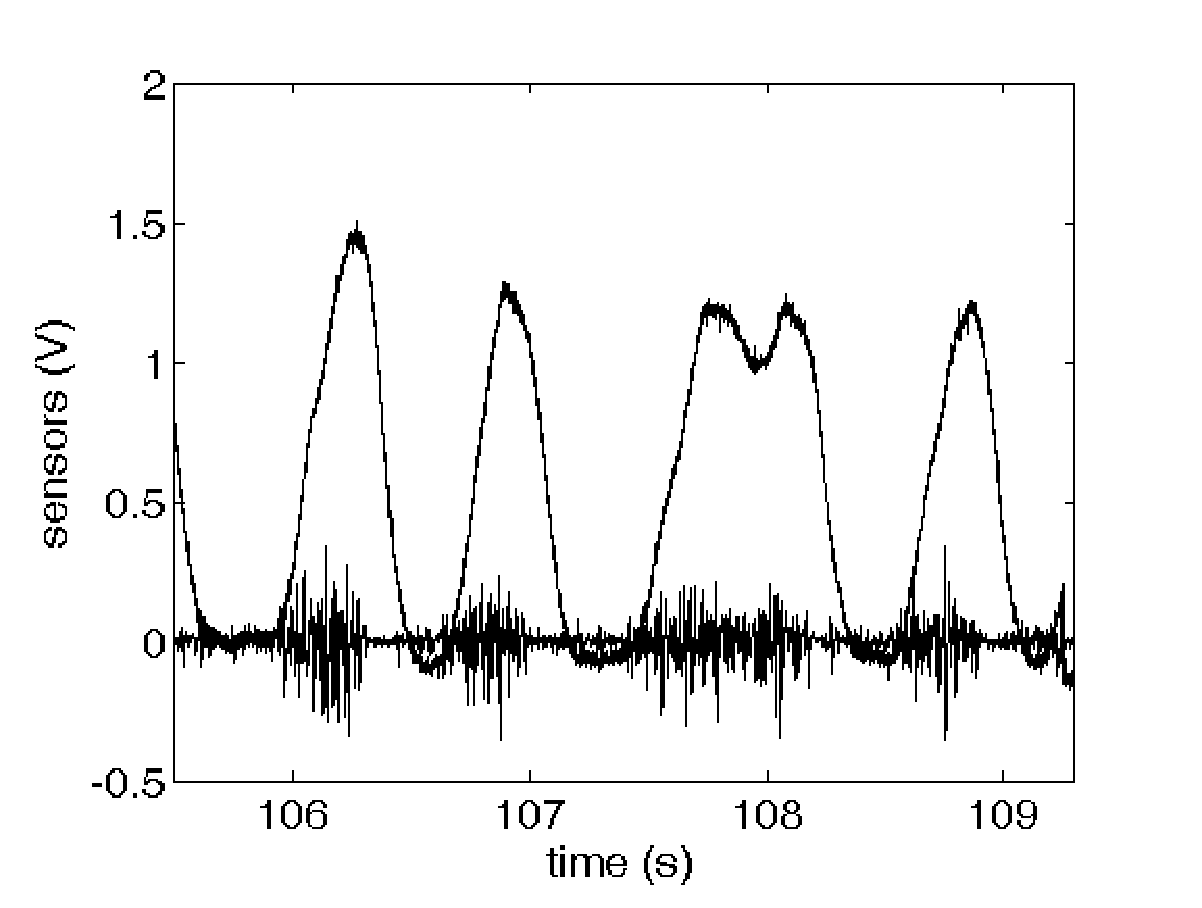
\includegraphics[width=0.45\textwidth]{force_raw.eps} &
%    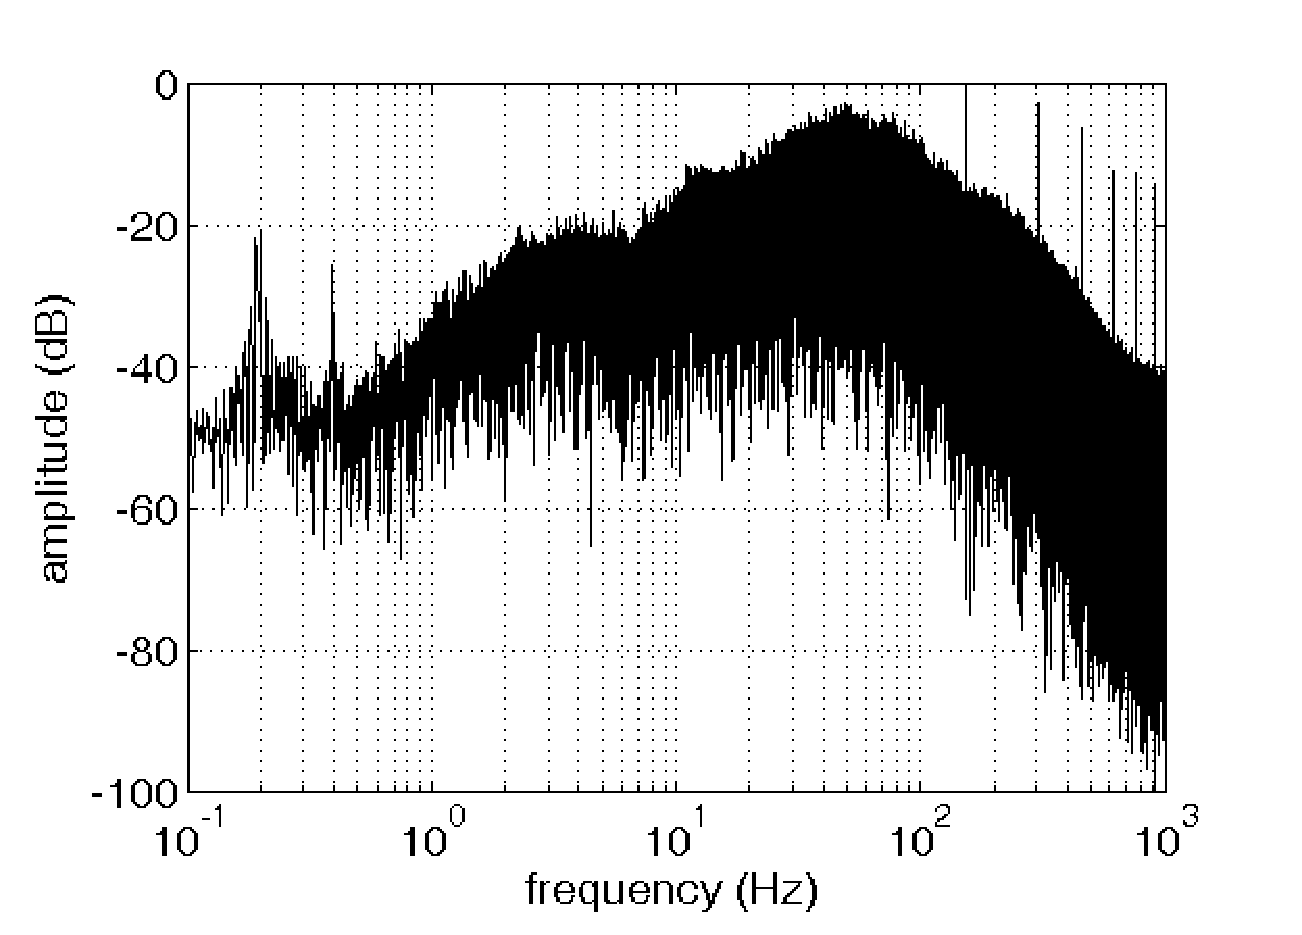
\includegraphics[width=0.45\textwidth]{spectrum_raw.eps} \\
%    $(a)$ & $(b)$ \\
%  \end{tabular}
%  \caption{$(a)$ typical raw EMG and force signals (the EMG signal
%    being the bottom, high-frequency one); $(b)$ frequency diagram of
%    the EMG signal.}
%  \label{fig:spectra}
%\end{figure*}

%\begin{figure*}[!ht] \centering
%  \begin{tabular}{ccc}
%    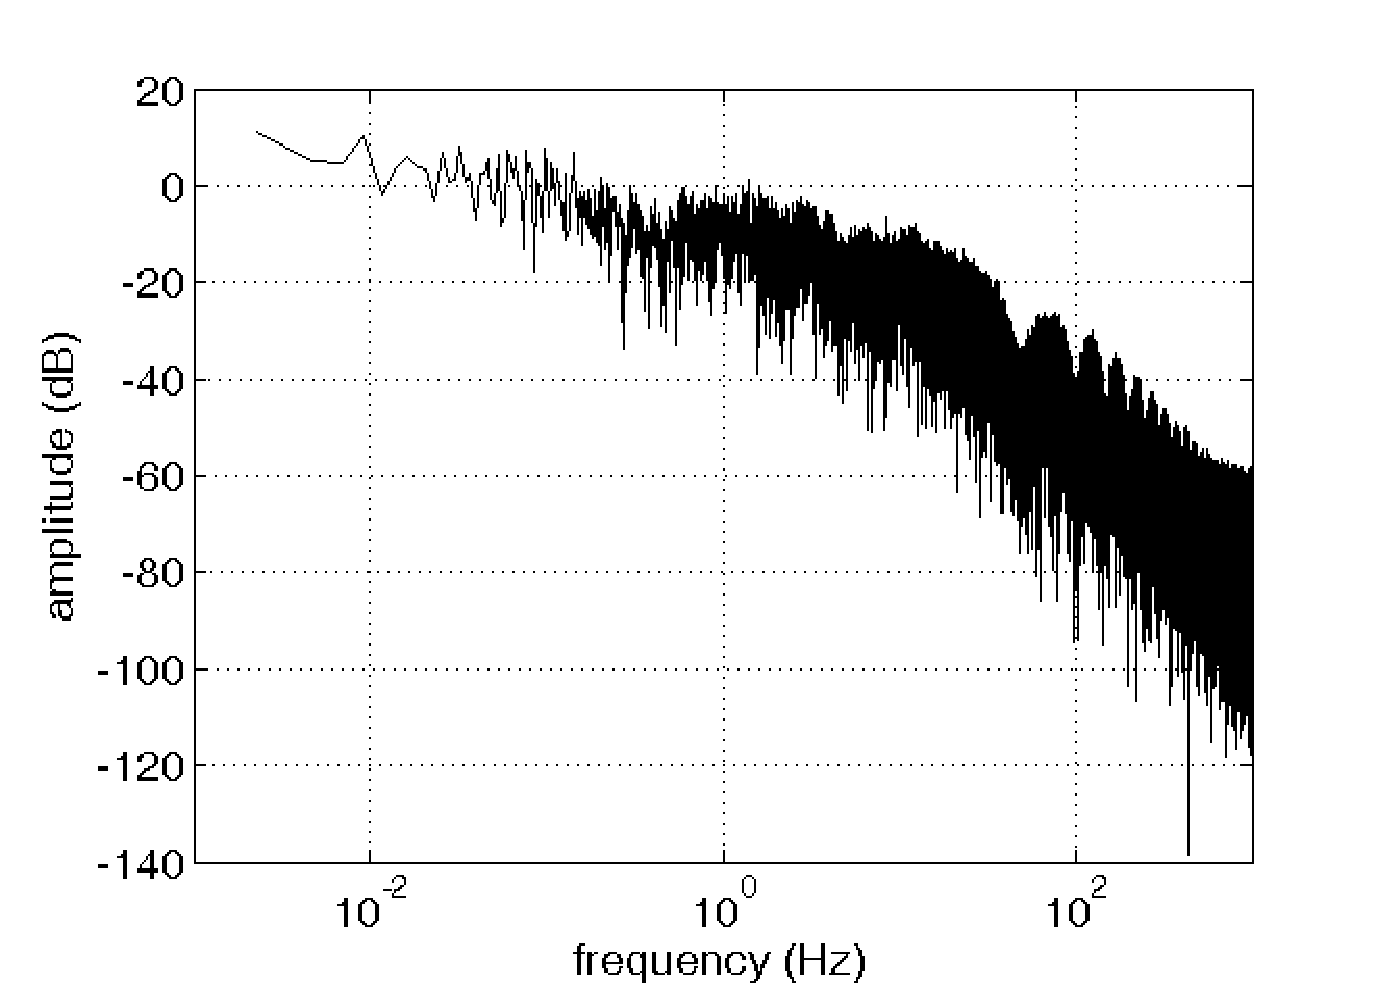
\includegraphics[width=0.3\textwidth]{spectrum_RMS0040.eps} &
%    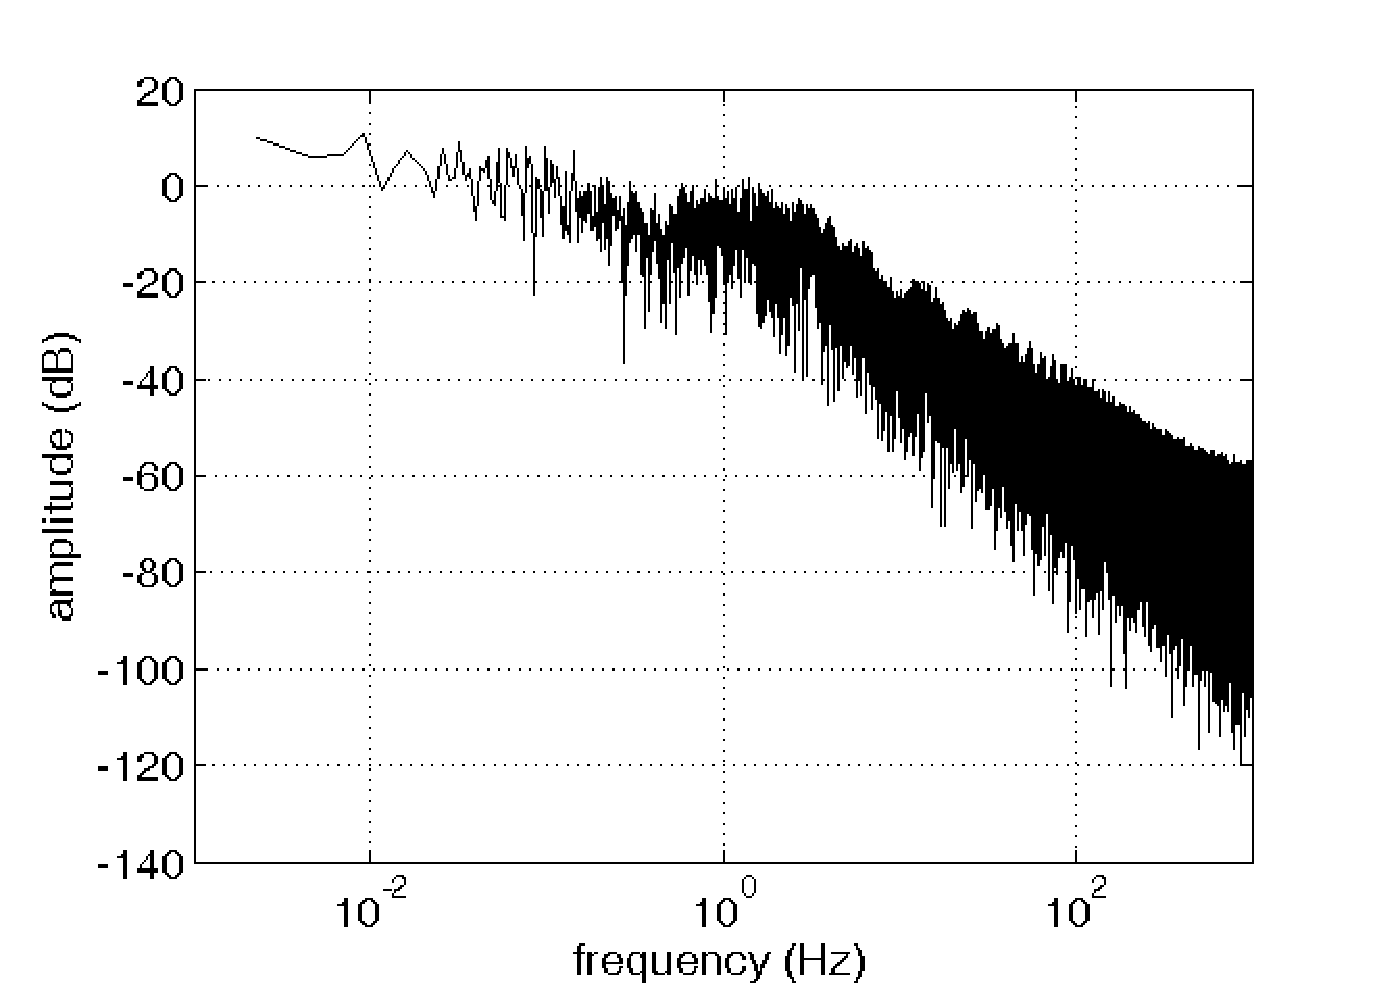
\includegraphics[width=0.3\textwidth]{spectrum_RMS0200.eps} &
%    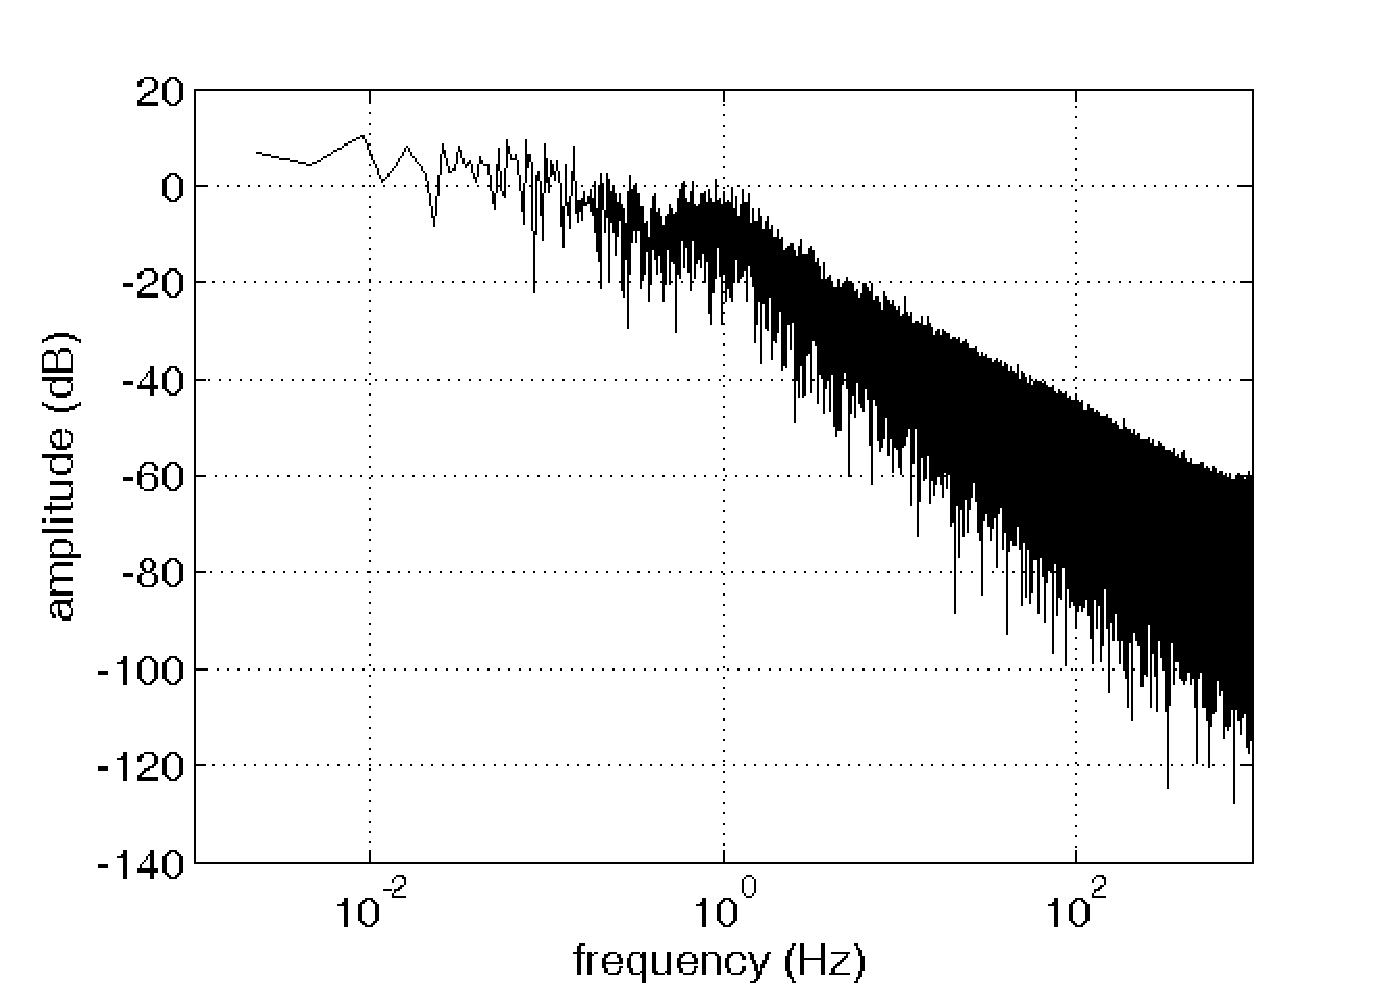
\includegraphics[width=0.3\textwidth]{spectrum_RMS1000.eps} \\
%    $(a)$ & $(b)$ & $(c)$ \\
%  \end{tabular}
%  \caption{(left to right) effects of the RMS on the bandwidth of the EMG
%    signals, for $T_{RMS} = 20, 100, 500ms$.}
%  \label{fig:RMSs}
%\end{figure*}

Figure \ref{fig:spectra} $(a)$ shows the typical EMG signal (red)
and force (blue) recorded by the force sensor. Clearly the
amplitude of the envelope of the EMG is related to the force, as is
indicated in literature. Panel $(b)$ of the Figure shows the bandwidth
of the EMG. Figure \ref{fig:RMSs} shows the effect of the RMS
on the frequency components of the EMG, for three different values of
$T_{RMS}$. In all cases, the RMS signal bandwidth is
upper-bounded by about $25$Hz (panel $(a)$, for $T_{RMS}=20ms$) to
$10$Hz (panel $(c)$, for $T_{RMS}=0.5s$), as expected (larger values
of $T_{RMS}$ correspond to a better filtering but also to a larger
delay). According to these figures, we subsampled the RMS of the EMG
signals at $25$Hz by taking one sample in $80$ of the original sequence,
resulting in about $30.000$ samples for each subject.

Lastly, samples for which the applied force was lower than a specific
threshold were removed. After verifying several choices both numerically
and visually, the threshold was uniformly set at $20\%$ of the mean force
value obtained for each subject and phase.

\subsection*{Statistical analysis}

According to previous literature (e.g., \cite{smagt,2008.BioCyb}), the
statistical analysis was carried on using Support Vector Machine (SVM).
For a comprehensive tutorial on SVMs refer to
\cite{Burges98,SmolaTut2004}. SVMs are a statistical learning method
able to build an approximated map between an input space and a label
(classification) or a real value (regression). Classification is here
used to classify the type of grasp according to the EMG signal,
whereas regression is used to understand how much force the subject is
exerting, independently from the grasp type. The input space is
$\RR^7$, one coordinate for each EMG electrode. We used the
ground truth values as labels and the force value given by the force sensor
for the regression. Notice that SVMs work here in real-time, associating a grasp type
and a force value to an EMG value at each instant of time.
Grasp type and forces are then predicted almost at the onset of the
grasping movement, differently from what happens in other approaches (e.g.,
\cite{smagt,Sebelius2005}) in which all values of the input signal over a
further time-window are employed as the input space.

In order to ease the computational burden we employed uniformisation
\cite{2008.BioCyb} to reduce the size of the training sets. The samples
in a training set are considered one by one in chronological order, as it
would happen in an on-line setting, and each new sample is added to the
training set if and only if its Euclidean distance from all training samples
retained so far is larger than a predefined value $d$. Values of $d$ were
set to $0.02$ for the SA phase and $0.032$ for the FA phase. These values
were chosen in order to get not more than one thousand training
samples for subject $1$. The choice is arbitrary, but notice that
(see \cite{2008.BioCyb} again) the performance of such
systems changes linearly as $d$ changes, whereas the training set size
varies polynomially; thus, it is always possible to find a
polynomially smaller training set, if needed, which will degrade the
performance only linearly. This really means that the initial choice
of $d$ is not crucial. Notice, too, that no testing sets have been
uniformised, in order to give a more realistic result.

SVM analysis was performed for each subject and for each phase,
to check how the performance depends upon subjects and conditions.
For classification, the performance index is, as is
customary, the percentage of overall correctly guessed labels. For
regression, the performance index is the correlation coefficient
evaluated between the predicted force signal and the real one. The choice
of the correlation coefficient is suggested by this consderation:
when driving a prosthesis we are
not interested in the absolute force values desired by the
user/subject, since mechanical hands usually cannot apply as much
force as human hands do, for obvious safety reasons\footnote{Or, e.g.,
in teleoperation scenarios, they could be able to apply \emph{much
more} force than a human hand can.}. We are rather concerned about
getting a signal which is strongly correlated with the user/subject's will.
Anyway, we also report about the normalised root mean-square error (NRMSE),
in order to give a broader view of the results. Normalisation is done against the
signals' ranges (notice, though, that correlation is the criterion used to
find the optimal parameters during grid search).

We employed a well-known freely available SVM package, \emph{libsvm}
v2.83 \cite{ChangL01}, in the Matlab wrapped flavour; the Gaussian kernel
was chosen, since it is a standard choice in previous literature.
EMG data were normalised along each dimension, as is customary, by subtracting
the mean value and dividing by the standard deviation. $5$-fold cross-validation was
used to assess the generalisation error for each training set; this measure
was then used for grid-searching the typical Gaussian kernel hyperparamters
of a SVM, called $\gamma$ and $C$. Once these parameters were found, the overall
performance was evaluated as the mean and standard deviation of the performances
obtained on each fold.

%To sum up, Figure \ref{fig:Algorithm} graphically depicts the structure of the
%system. Notice that there can actually be two different RMS windows, one for
%classification and one for regression.

%\begin{figure*}[!ht] \centering
%  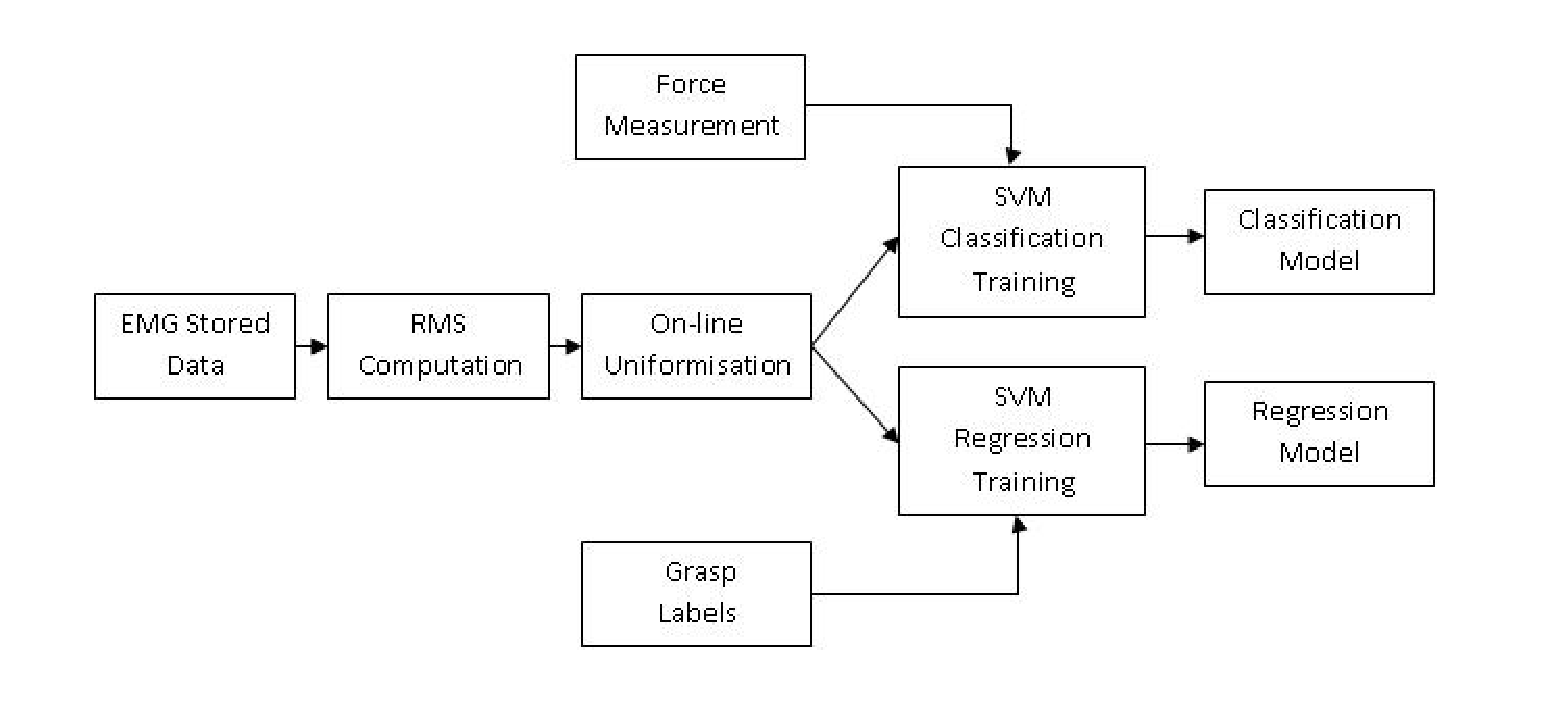
\includegraphics[width=0.75\textwidth]{Schema.eps} \\
%  \caption{Graphical representation of the system employed to solve our problem.}
%  \label{fig:Algorithm}
%\end{figure*}

\section*{Results}
\label{sec:exp}

\subsection*{Per-Subject Analysis}

%\begin{figure*}[!ht] \centering
%  \begin{tabular}{cc}
%    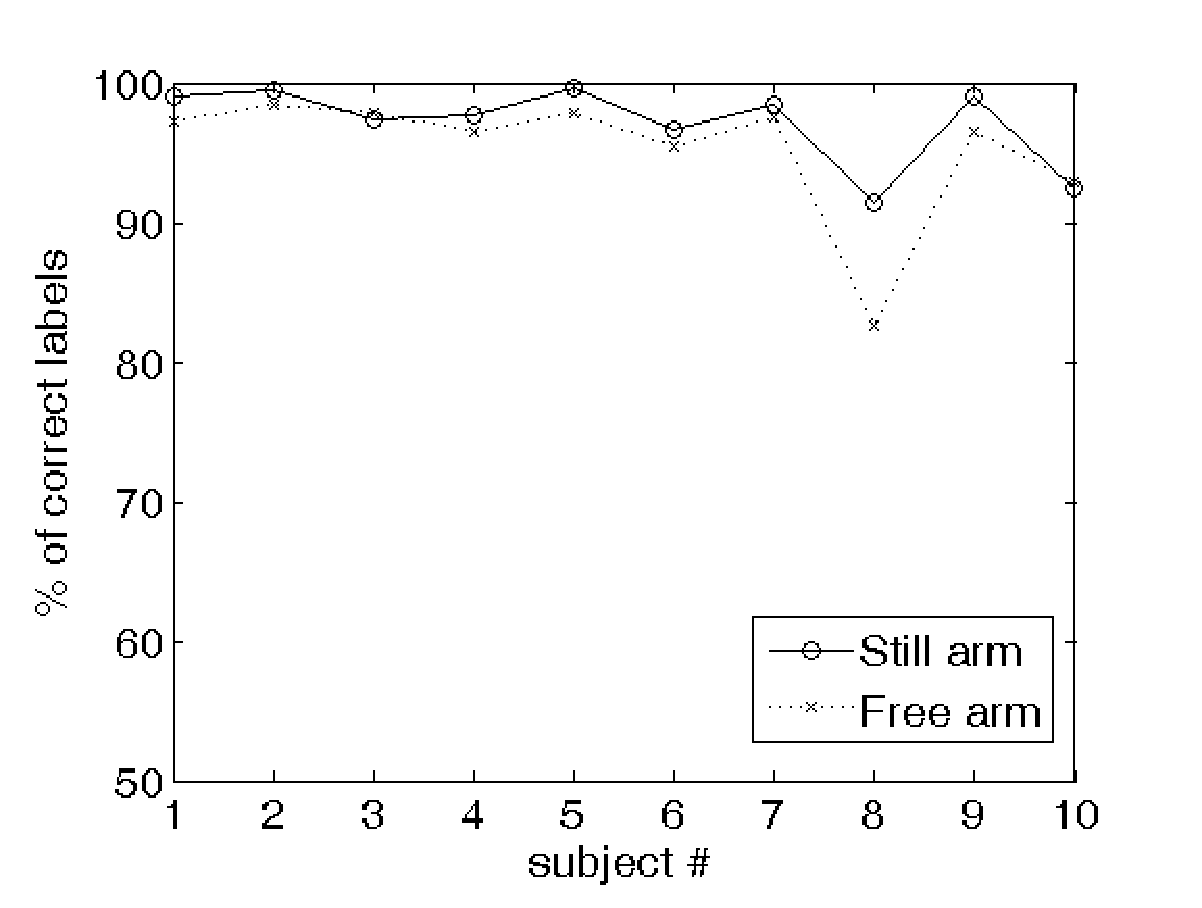
\includegraphics[width=0.45\textwidth]{perfClass.eps} &
%    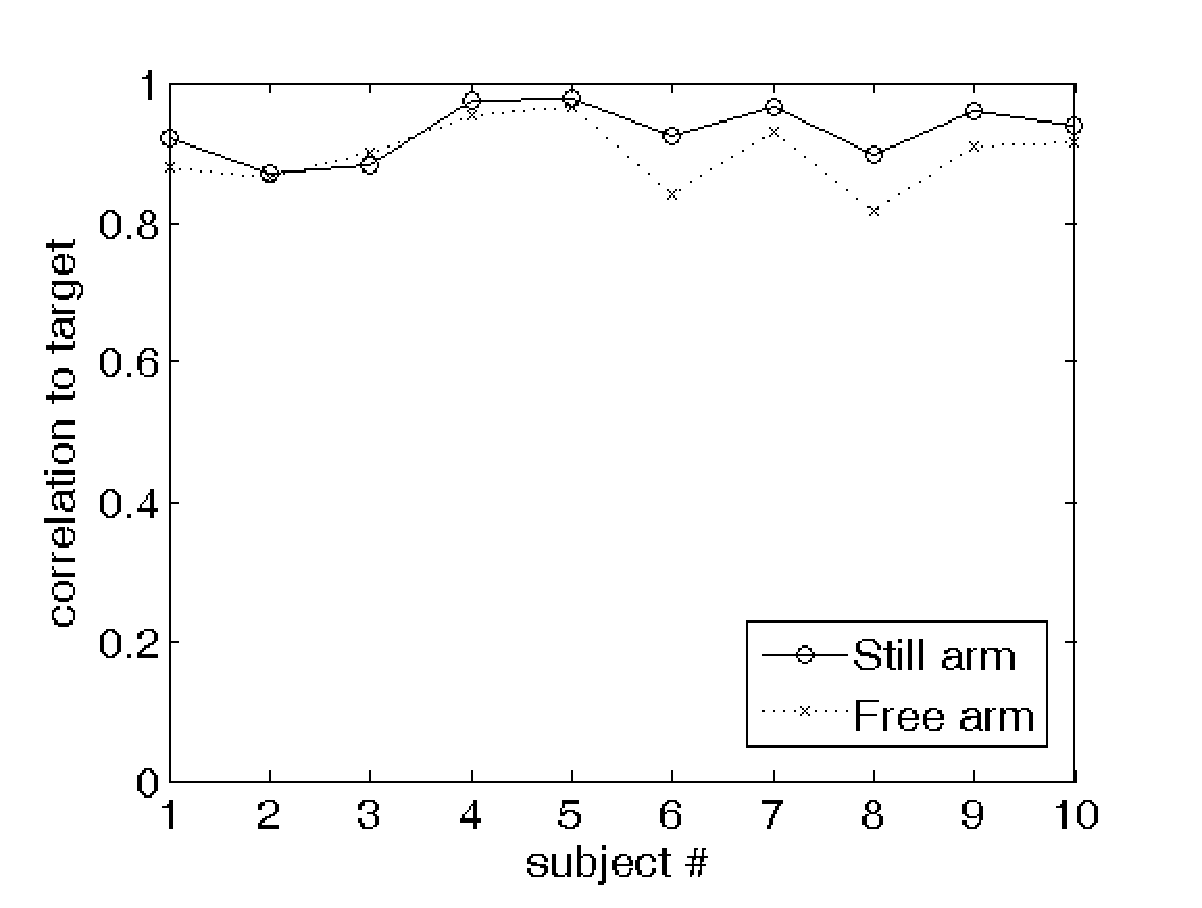
\includegraphics[width=0.45\textwidth]{perfRegr.eps} \\
%    $(a)$ & $(b)$ \\
%  \end{tabular}
%  \caption{classification $(a)$ and regression $(b)$ results obtained
%    by the system, on both phases of the experiment (FA and SA) and
%    for each subject.}
%  \label{fig:results}
%\end{figure*}

Figure \ref{fig:results} shows the main results. Classification
accuracy (top panel) for the SA phase ranges
from $99.58\% \pm 0.17\%$ (subject $5$) to $91.37\% \pm 0.89\%$ (subject $8$);
for the FA phase, it ranges
from $98.40\% \pm 0.08\%$ (subject $2$) to $82.43\% \pm 1.24\%$ (subject $8$ again).
On average over all subjects, the classification accuracy is
$97.14\% \pm 2.90\%$ for SA and $95.24\% \pm 4.77\%$ for FA.
Notice that the performance is
consistent by subject and by phase, meaning that $(a)$ hard subjects
in the SA phase are hard as well in the FA phase and viceversa, and
$(b)$ the FA phase is always harder than the SA phase.

Regression figures (middle and bottom panels) show that for the SA phase
the correlation to true signal ranges from
$0.9784 \pm 0.0017$ (subject $5$) to $0.8959 \pm 0.0033$ (subject $8$),
whereas for the FA phase it ranges from
$0.9657 \pm 0.0022$ (subject $5$) to $0.8161 \pm 0.0078$ (subject $8$).
On average, the correlation is $0.93 \pm 0.04$ for the SA phase and
$0.90 \pm 0.05$ for the FA phase. Again, consistency by subject and by
phase appears. Remarkably,
not all subjects which are slightly harder for regression (namely,
$1,2,3,6,8$) happen to be hard for classification; in particular, only
subject $8$ is definitely hard \emph{both} for classification and
regression, while, e.g., subject $6$ is hard for regression but not
that hard for classification. The bottom panel shows that an analogous
situation appears if we consider the NRMSE. (Recall that the NRMSE is
an error measure while the correlation to target is a positive performance
index.)

Figure \ref{fig:examples} shows the real and guessed force values for a
typical subject, namely number $6$, FA phase. Strong correlation between
the guessed and true values is visually apparent, in agreement with the
performance values outlined before.
On the other hand, Figure \ref{fig:confusion} shows the (average)
confusion matrices for the SA and FA phases. Clearly, most of the classification
errors, for both phases, regard the ``power grasp'' being mistaken for the
``other fingers precision grip''. This is intuitively sensible, since gripping
with middle, ring and pinkie finger involves co-contracting the index finger too.
This makes the former grip quite similar to the latter, from a muscular point
of view.

%\begin{figure*}[!ht] \centering
%  \begin{tabular}{cc}
%    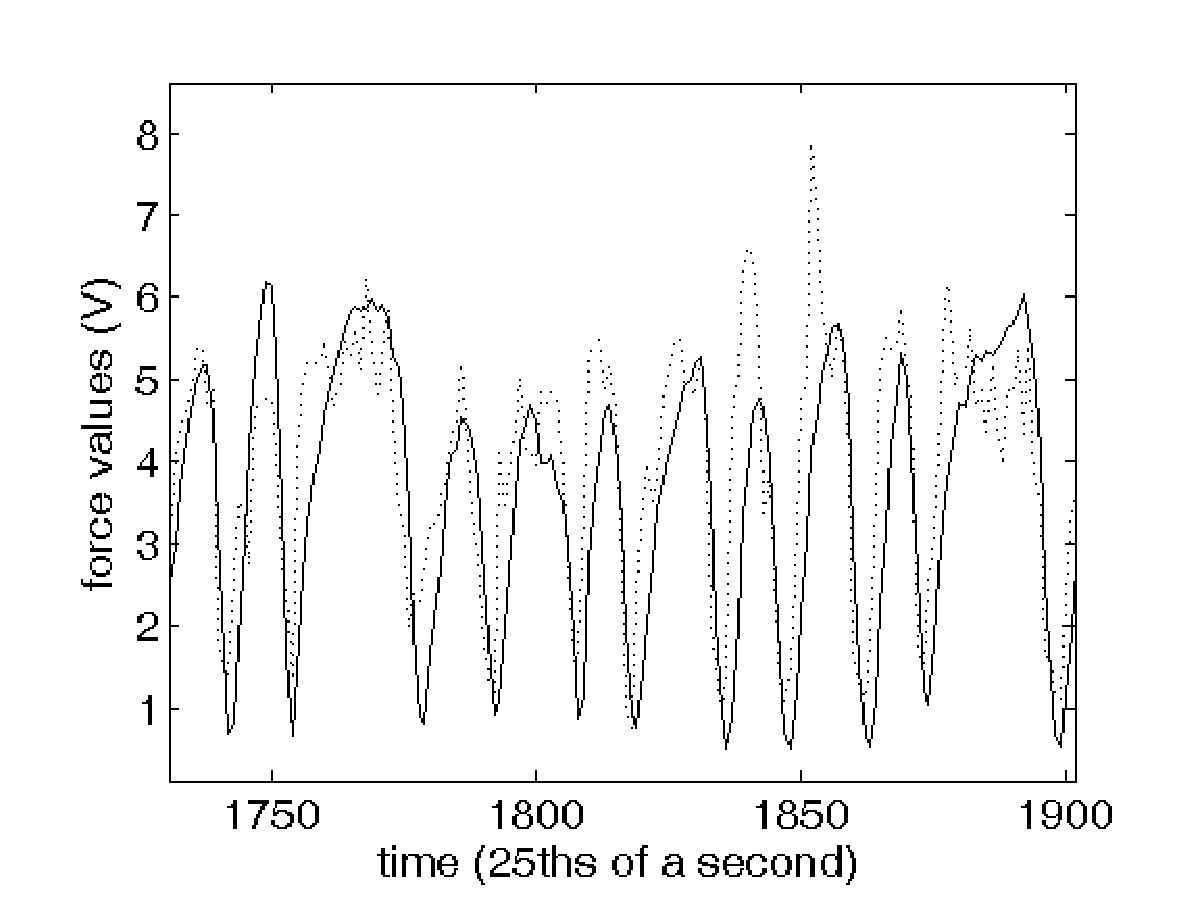
\includegraphics[width=0.45\textwidth]{example_6_one.eps} &
%    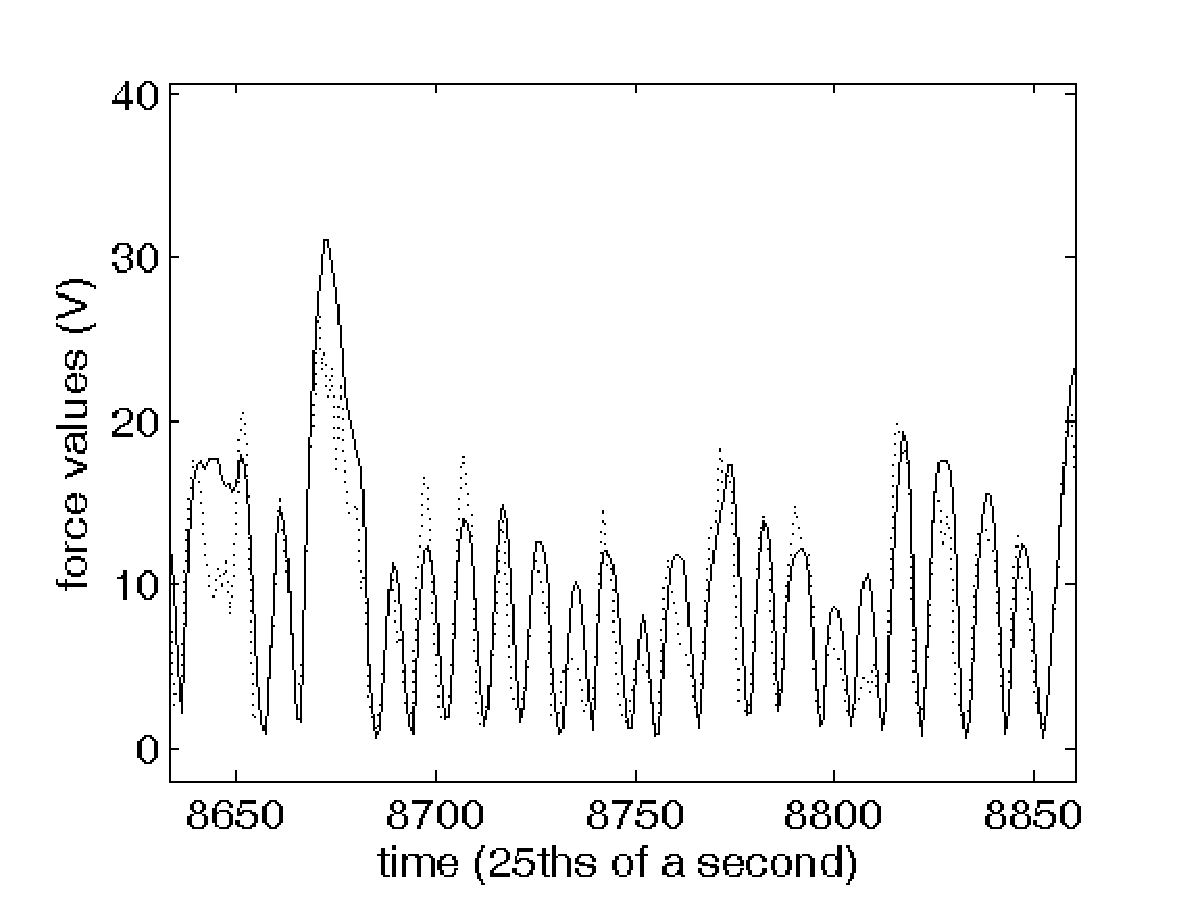
\includegraphics[width=0.45\textwidth]{example_6_two.eps} \\
%    $(a)$ & $(b)$ \\
%  \end{tabular}
%  \caption{comparing true (continuous line) and guessed (dotted line) force values for regression of a
%    typical subject (number $6$, FA phase).}
%  \label{fig:examples}
%\end{figure*}

%\begin{figure*}[!ht] \centering
%  \begin{tabular}{cc}
%    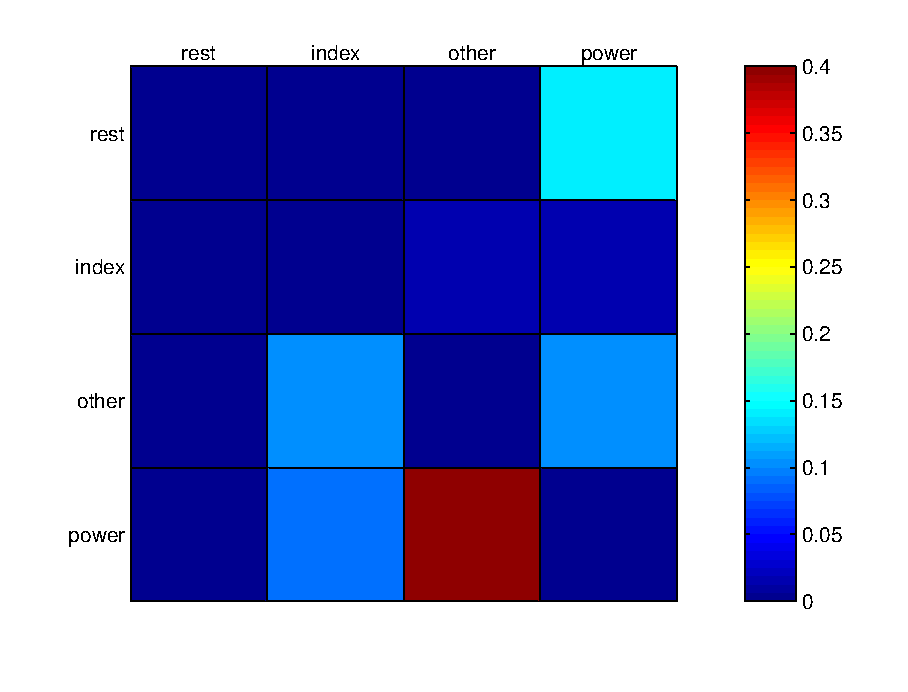
\includegraphics[width=0.45\textwidth]{confMat_1.eps} &
%    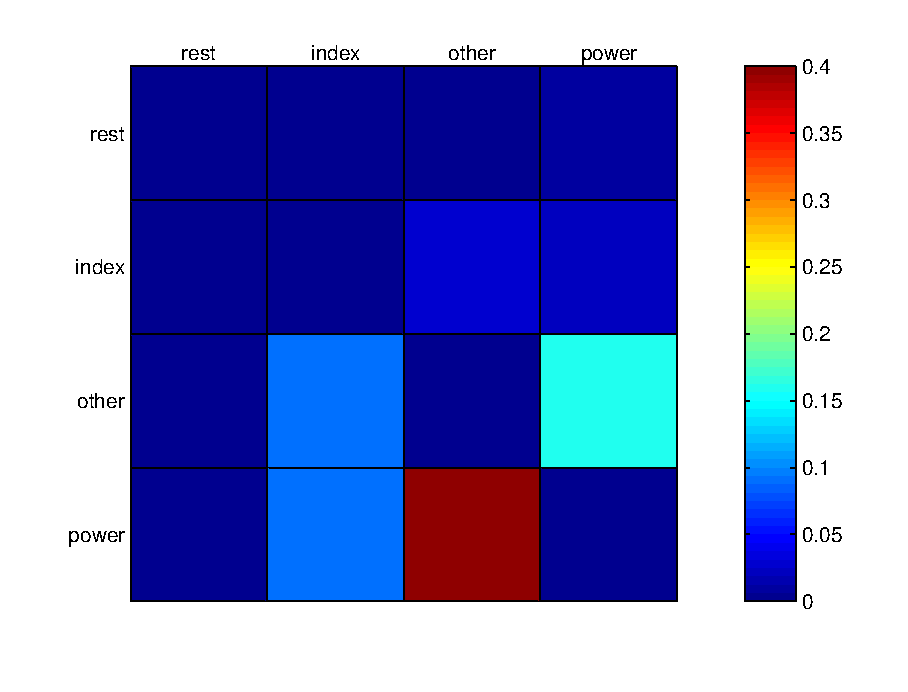
\includegraphics[width=0.45\textwidth]{confMat_2.eps} \\
%  \end{tabular}
%  \caption{confusion matrices for the SA phase (left) and FA phase (right). Each matrix
%           is the average over the confusion matrices of the $10$ subjects. A confusion
%           matrix $C$ is such that its $(i,j)$th element is the fraction of $i$ labels
%           mistaken for $j$ labels, over the total mistaken labels.}
%  \label{fig:confusion}
%\end{figure*}

To check whether there are any regularities among the subjects and phases,
we show in Table \ref{tab:hyp} the average values of (the logarithms of)
$\gamma$ and $C$ for the optimal models obtained via cross-validation
(knowing that a hyperparameter takes mostly a certain can narrow down the
grid search with new subjects).
The grid search ranges were $[0,3]$ for $log_{10}(C)$ and
$[-1.85,0.16]$ for $log_{10}(\gamma)$ (these are standard values in
literature, given the dimensionality of the input space). The average value of
$log_{10}(C)$ is around $1.5$, but its standard deviation is too wide
to allow narrowing the grid search, at least in the case of
classification. The standard deviation is smaller for regression than
for classification in both cases, which seems to indicate that
regression as a problem is more stable with respect to the
hyperparameters.

In order to check whether the FA phase is really indicative of what
a patient might do in her/his DLAs, we have trained a
machine on the data gathered during the FA phase and then tested it
on the data gathered during the SA phase. Figure \ref{fig:2on1} shows the
results of testing FA-models on SA data, and viceversa.

%\begin{figure*}[!ht] \centering
%  \begin{tabular}{cc}
%    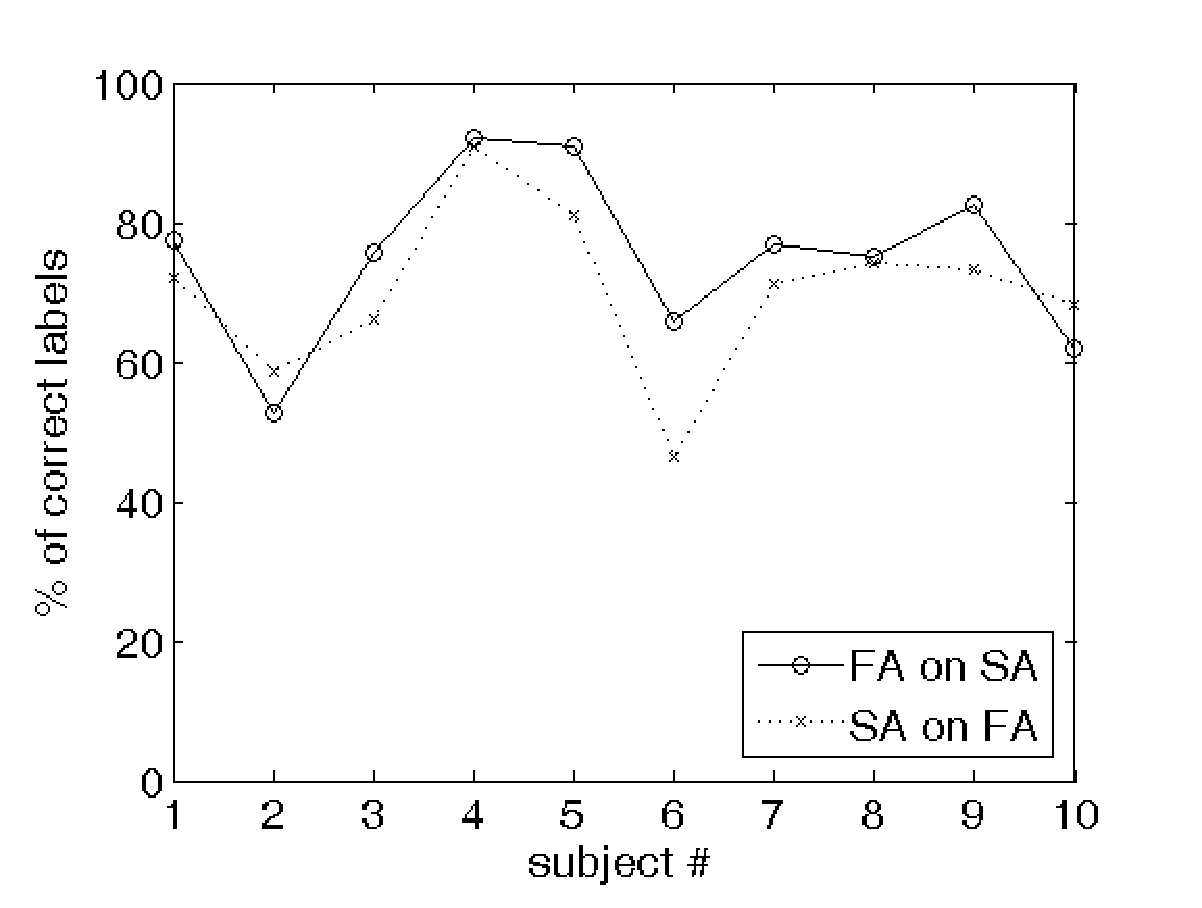
\includegraphics[width=0.45\textwidth]{2on1_class.eps} &
%    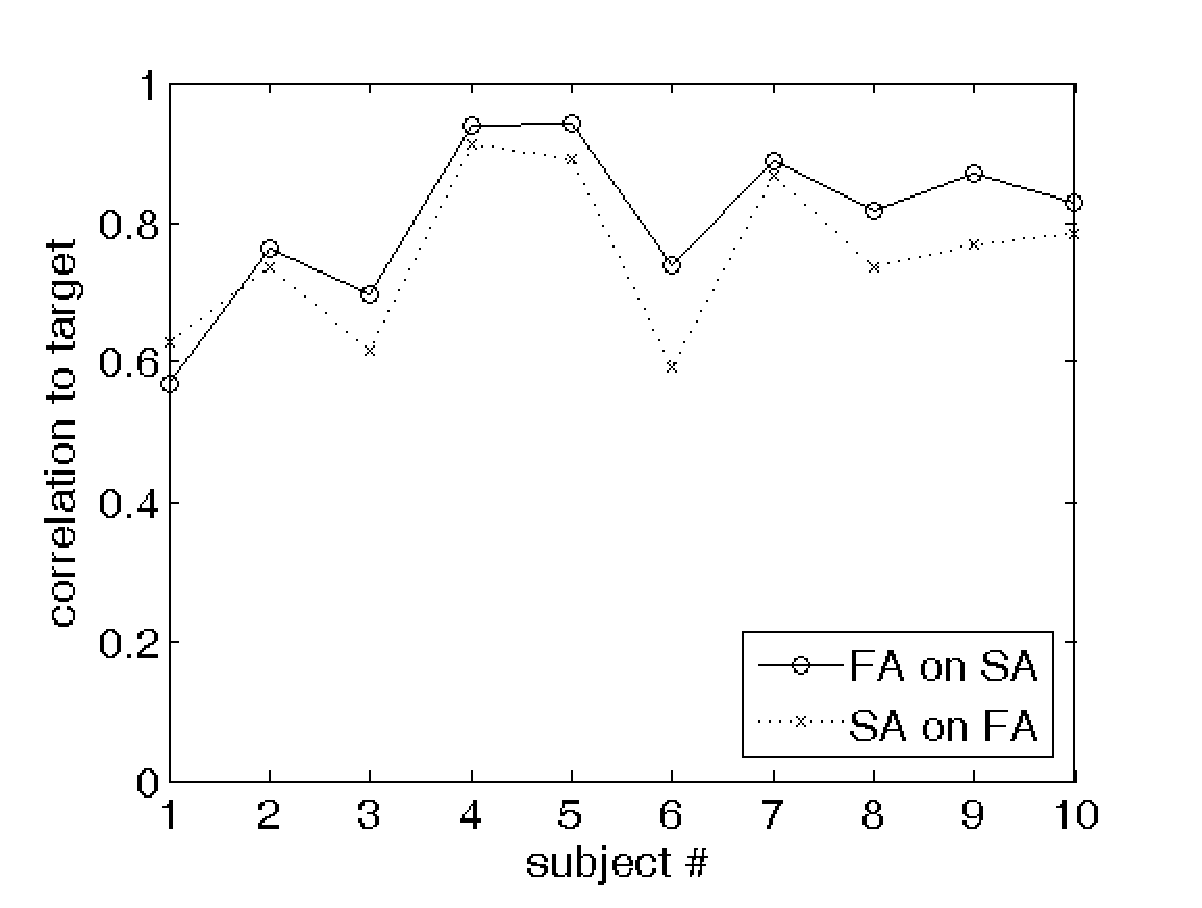
\includegraphics[width=0.45\textwidth]{2on1_regr.eps} \\
%    $(a)$ & $(b)$ \\
%  \end{tabular}
%  \caption{classification $(a)$ and regression $(b)$ results obtained
%    testing on SA-data models trained on FA, and vice-versa.}
%  \label{fig:2on1}
%\end{figure*}

FA-models tested on SA data obtain an average accuracy of $75.11\% \pm 12.34\%$
for classification and $0.8056 \pm 0.1151$ for regression;
whereas testing SA-models on FA data gives $70.17\% \pm 11.99\%$ in classification
and $0.7530 \pm 0.1153$ in regression. The advantage of FA models over SA models
is apparent, uniform and consistent. Notice that here we show no error bars,
since, for each subject and phase, there is just one training set and one testing set.

Lastly, let us consider the worst result of the per-subject analysis
--- subject $8$ in the FA phase, as far as classification is concerned.
One of the possible causes of this comparatively low performance
($82.43\% \pm 1.24$) is that too many samples are missing from the
original training set ($d$ too high). In order to test this hypothesis,
we let $d$ linearly range around the pre-set value of $0.032$ and check
$(a)$ the size of the resulting training set and $(b)$ the performance
obtained by the system. Figure \ref{fig:subj8} shows the result of
this test.

%\begin{figure*}[!ht] \centering
%  \begin{tabular}{c}
%    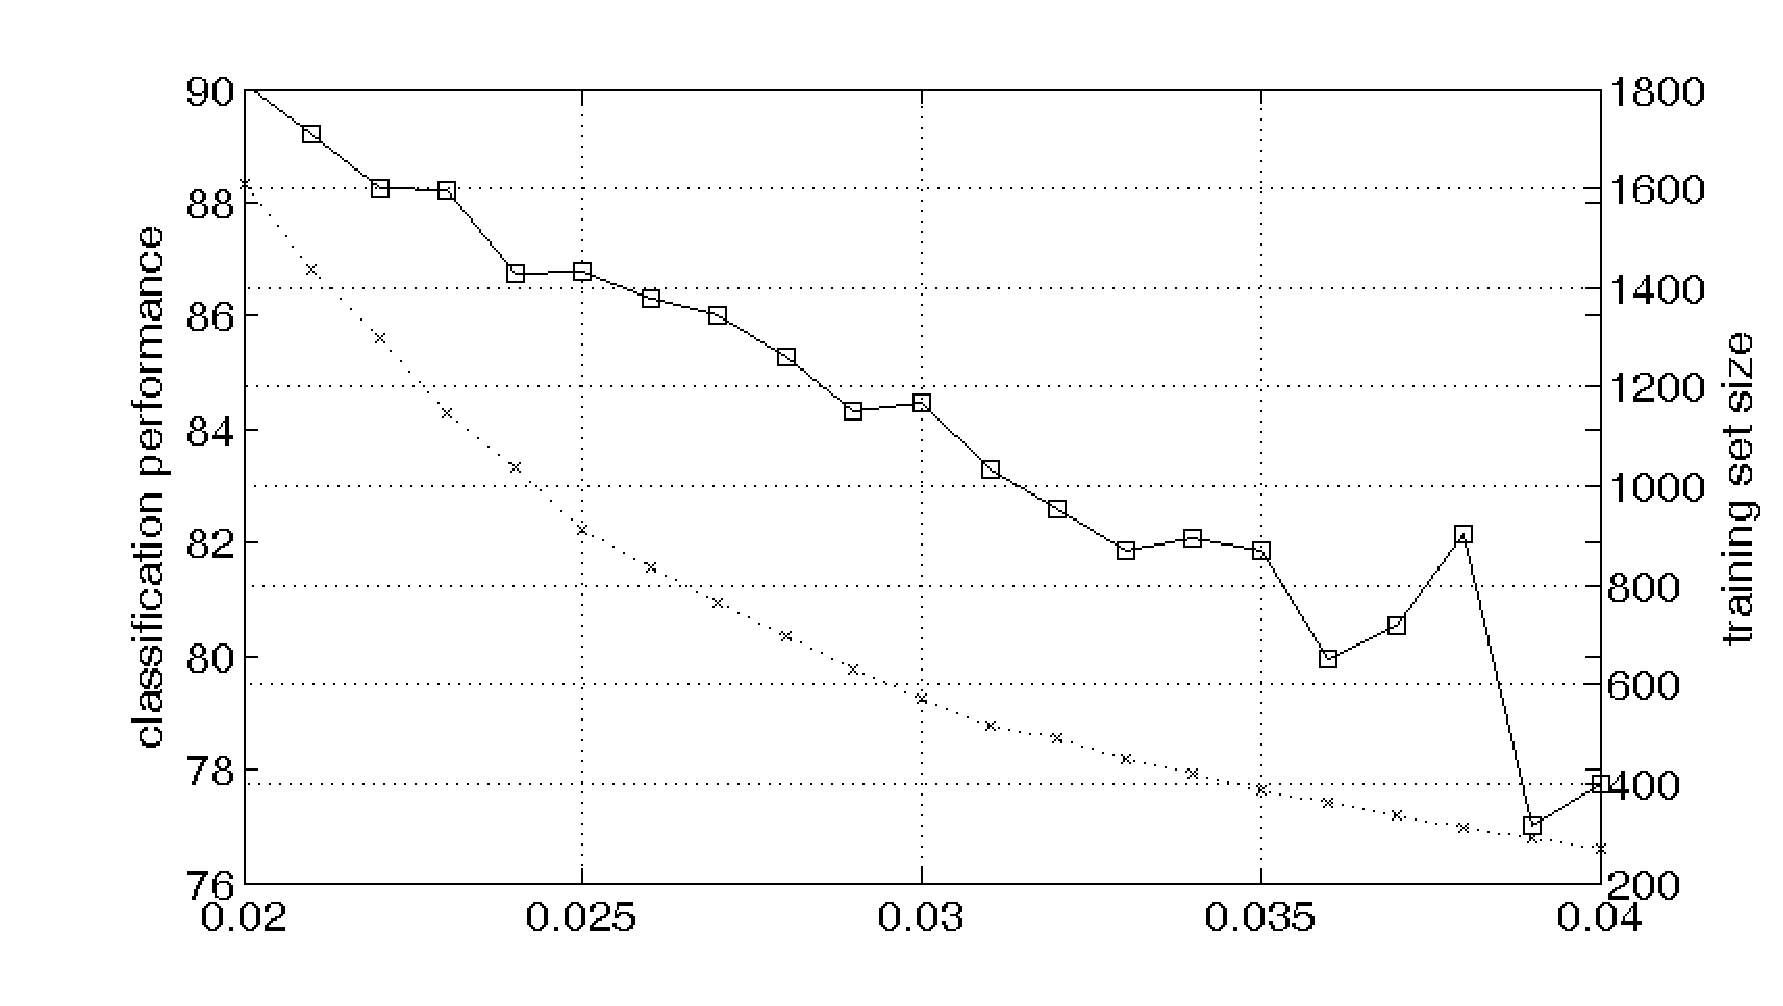
\includegraphics[width=0.6\textwidth]{subj8.eps} \\
%  \end{tabular}
%  \caption{size of the training set (dotted line) and classification
%    performance (continuous line), of subject $8$ in the FA phase, as
%    $d$ changes.}
%  \label{fig:subj8}
%\end{figure*}

The Figure confirms that the training set size has a decreasing
polynomial trend, while the performance changes linearly
\cite{2008.BioCyb}. In
particular, for $d=0.032$ the previously shown performance appears,
whereas if a larger performance is required, one can increase the
number of samples in the training set, or, which is equivalent, reduce
the magnitude of $d$. For instance, to get an accuracy of about $90\%$
$d$ must be set at $0.2$ ending up in a training set with some $1600$
samples.

\subsection*{Cross-Subject Analysis}

Recall that in this experiment, for all subjects, the EMG electrodes
were carefully positioned on the forearm according to an anatomical
guideline, meaning that noise due to inter-arm differences should be
to some extent avoided. We can therefore check how well each model
performs on each subject by building a cross-subject performance
matrix $A$, for both classification and regression, and for both phases,
in which $A_{ij}$ is the performance index attained by a model trained
on data gathered from subject $i$ while predicting data gathered from
subject $j$.  Figure \ref{fig:cross} shows the matrices.

%\begin{figure*}[!ht] \centering
%  \begin{tabular}{cc}
%    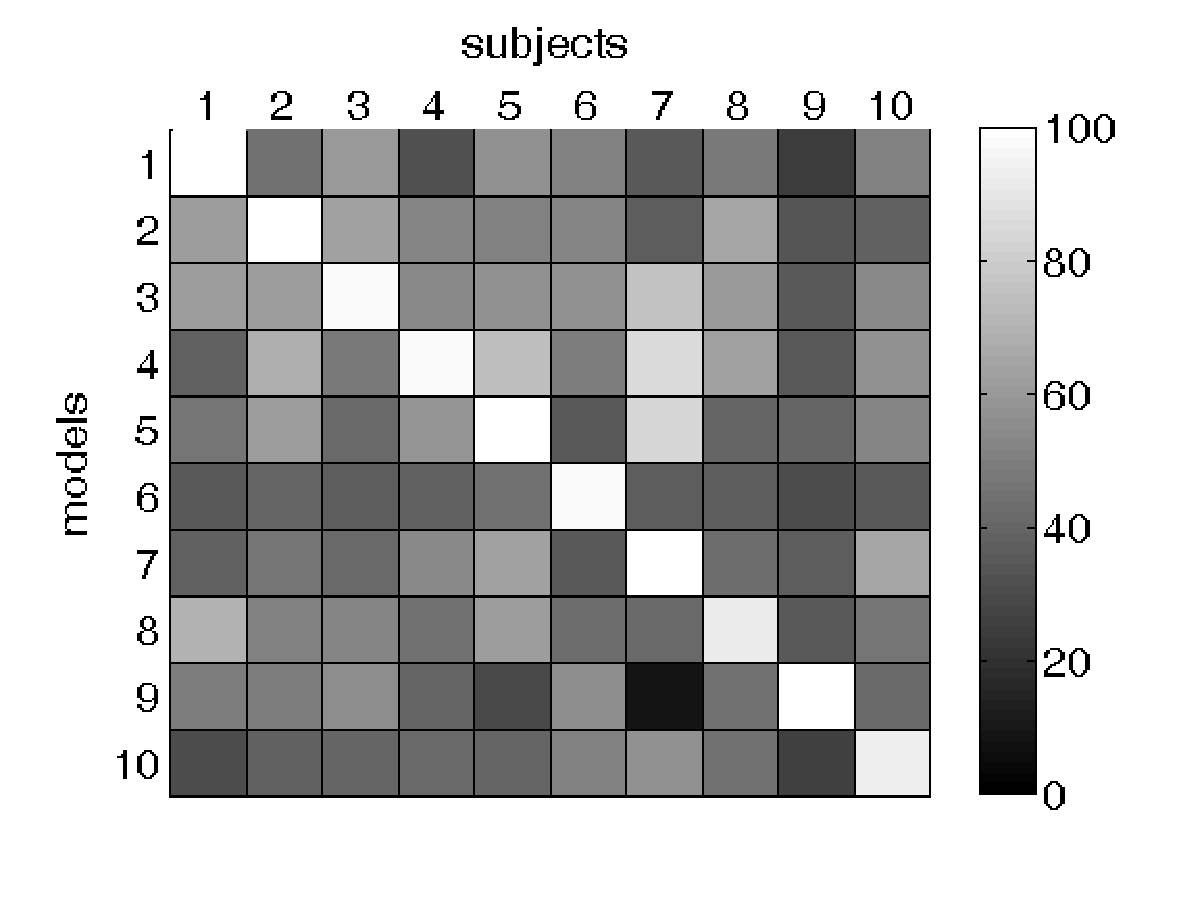
\includegraphics[width=0.45\textwidth]{crossClass1.eps} & 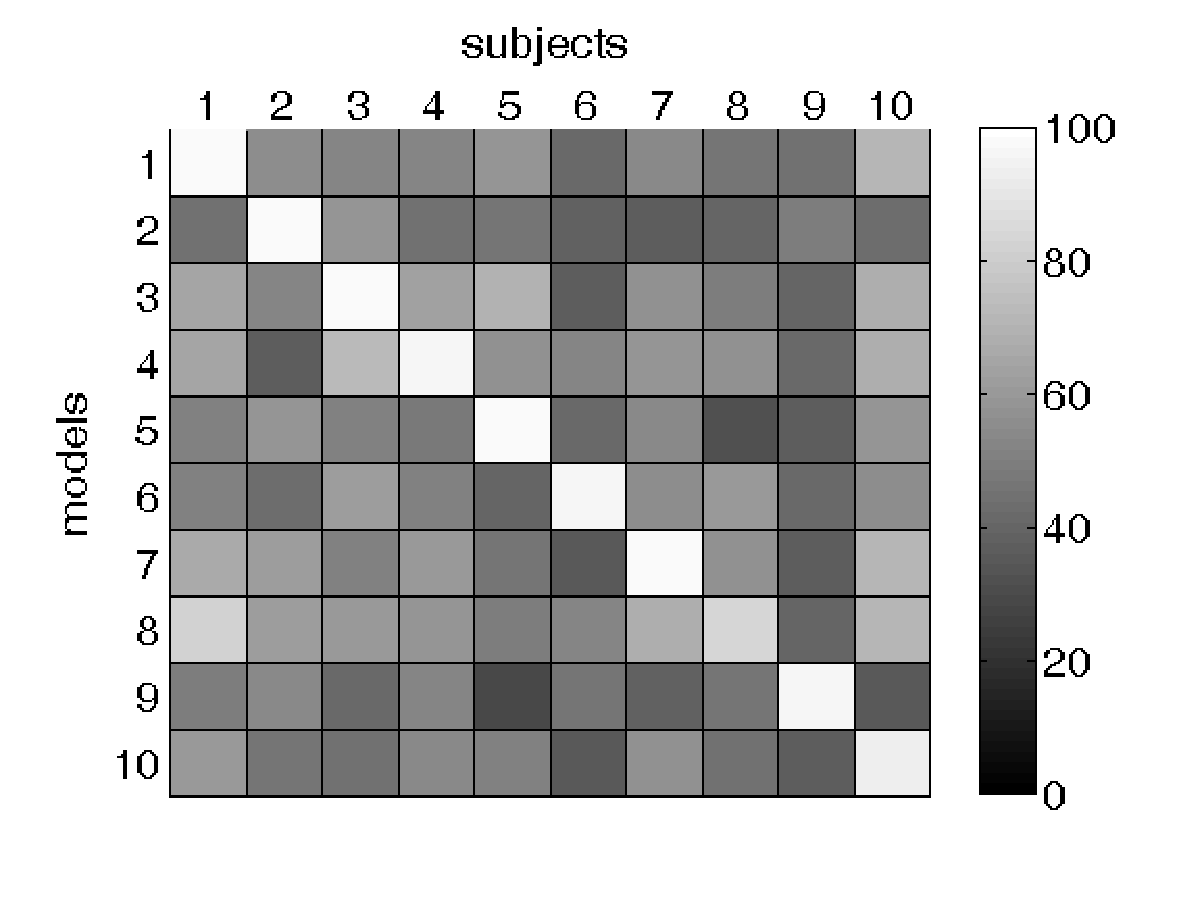
\includegraphics[width=0.45\textwidth]{crossClass2.eps} \\
%    $51.69\% \pm 19.27\%$ & $54.04\% \pm 16.42\%$ \\
%    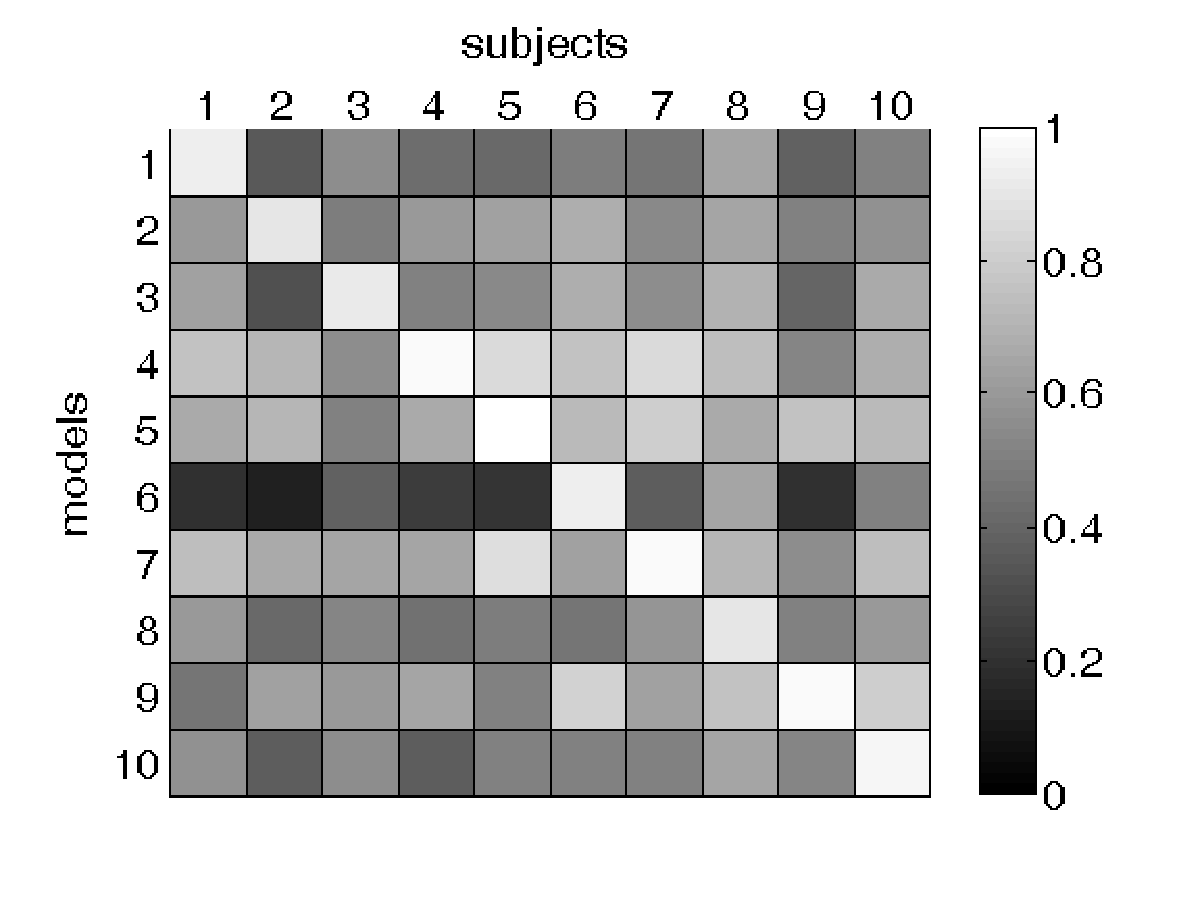
\includegraphics[width=0.45\textwidth]{crossRegr1.eps} & 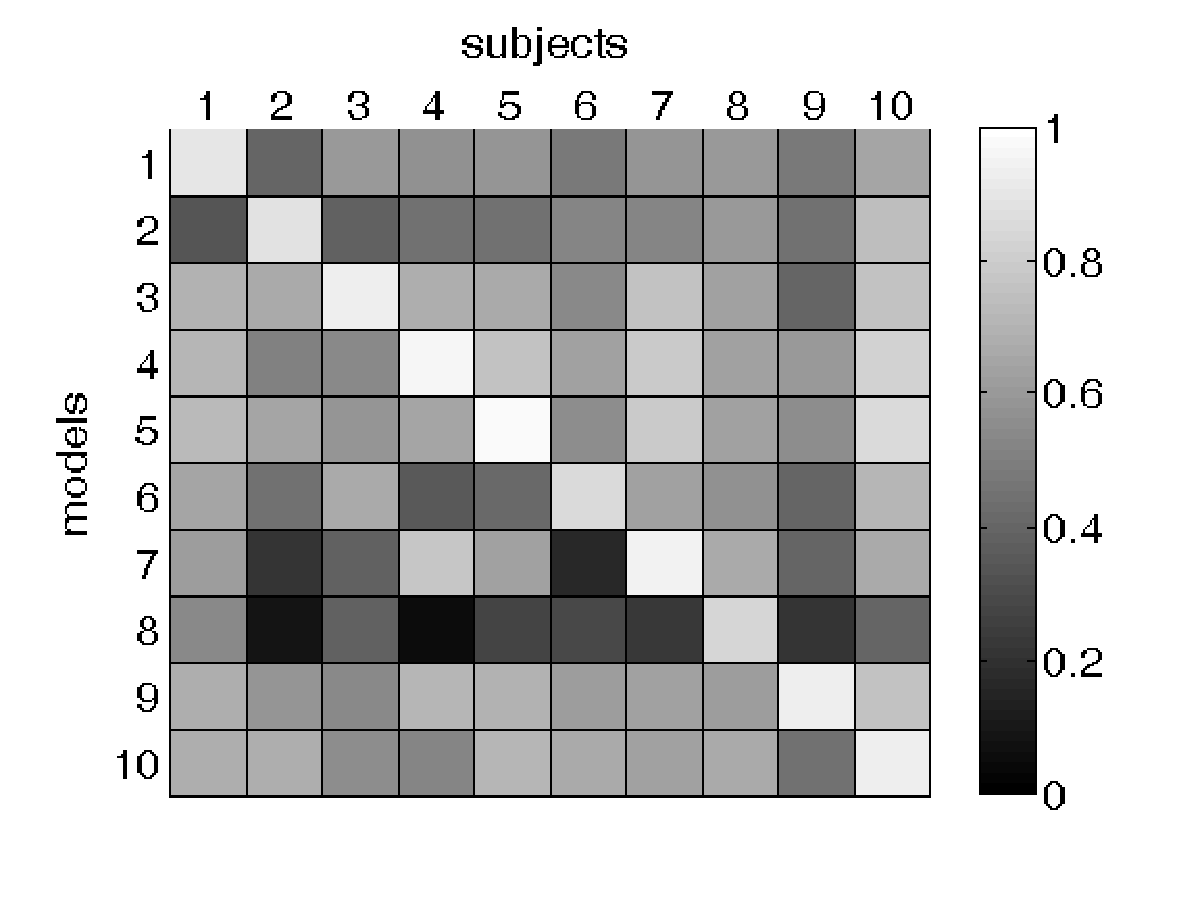
\includegraphics[width=0.45\textwidth]{crossRegr2.eps} \\
%    $0.60 \pm 0.18$ & $0.58 \pm 0.19$ \\
%  \end{tabular}
%  \caption{cross-subject performance matrices, for classification (top
%    row) and regression (bottom row), in the SA (left column)
%    and FA phase (right column); the numbers refer to all element of
%    the matrices, excluding the diagonals.}
%  \label{fig:cross}
%\end{figure*}

The overall results indicate that a large amount of the models
overlap, or at least that there is a certain cross-subject capacity of
prediction. Consider the numbers below the matrices in the Figure: in
classification, the performances are $51.69\%$ and $54.04\%$, with the
remarkable particular that the FA-models are slightly, but
consistently, \emph{better} in cross-subject analysis (higher mean
values and lower standard deviations) than the SA-models. As far as
regression is concerned, the average cross-subject correlation is
around $0.60$. Notice that models trained
on subjects $6$ (for the SA phase) and $8$ (FA phase) appear to be
particularly bad in predicting other subjects' data (the related rows
of the bottom left and right matrices, in turn, are rather darker than
the average).

In previous work it was shown that a significant (inverse) correlation
appears between the cross-subject performance matrices and the
\emph{cross-distance matrices} $D$,
obtained by evaluating a mean distance $D_{ij}$ between
two sample sets $S_i$ and $S_j$ like this:

$$ D_{ij} = \frac{1}{|S_j|} \sum_{s_j \in S_j}{\min_{s_i \in S_i}{ ||s_j-s_i||^2 } } $$

This analysis for each pair $(i,j)$ of subjects and for
the two phases and problems shows that inverse correlation
is absent in the case of the FA phase in classification; it is mild
($-0.32$) for SA in classification; and that it is strong in the case
of regression ($-0.63$ for the SA phase and $-0.65$ for the FA
phase). It is likely that the correlation in regression is connected
to the actual smoothness of the function the system is trying to
approximate. It is unclear why the classification problems show a
weak correlation or none at all.

\section*{Discussion and Conclusions}
\label{sec:discussion}

Several authors, even of this very work, have already assessed that
machine learning methods, applied to this problem, can solve it (an
incomplete list includes
\cite{chan2005,tsukamoto,englehart08,cipriani,2008.BioCyb}). The
research is all the more interesting since very recent work on
amputees, both from the neuroscientific \cite{sirigu1,sirigu2}
and the engineer's \cite{sebelius,2009.JPP,ramos}
point of view, clearly shows that it is applicable to the disabled.

Within this stream of research, in this work we aimed at answering
these questions:

\begin{enumerate}

  \item can forearm surface EMG be successfully applied to any (healthy) subject?

  \item will it work in Daily-Life Activities?

\end{enumerate}

The first question is tantamount to asking whether a uniformly good
performance can be obtained for each subject; the second question is
equivalent, in our framework, to asking whether the performance is
comparable between the SA and FA phases, provided that we agree upon
considering the FA phase as a reasonable experimental proxy of DLAs
of the standard patient. Our results point at a positive answer to
both questions.

Firstly, the figures obtained by our approach on the SA phase are
comparable to those found in other, related work such as
\cite{ramos,cipriani} or \cite{2008.BioCyb} where the predicted signals
were actually used to control the DLR-II hand in real-time. This
indicates that the approach will reasonably work on any healthy subject.
Combining this result with the more recent results obtained on amputees
listed above, we conclude that the approach is viable for a wide range
of patients, too. On the other hand, we are not claiming that SVMs are the one and only
good method. At least neural networks, LWPR \cite{lwpr} and Hidden Markov
Models \cite{chan2005} have been employed too, with similar results; probably,
even simpler approaches would get an acceptable level of performance,
which further raises the hopes for a real system based upon these
results. From the point of view of machine learning, interpreting surface
EMG is an easy task, a feeling corroborated, at least in the case of
regression, by the uniformity of the optimal hyperparamters found by
grid search.

Secondly, we can state that the approach also works while the subjects
are engaged in non-controlled activities; the results obtained in the
FA phase are in the same order of performance as those in the SA phase.
A deeper analysis reveals that FA models are in a sense ``wider'' than
SA ones, since they test better on SA data than the reverse.

As a side result, we notice that uniformisation can produce remarkably
small training sets (some $30$ times smaller) which nevertheless can be
used to generate models with excellent accuracy, and we confirm
the phenomenon described in \cite{2008.BioCyb}: as the minimum distance
$d$ is linearly increased, performance degrades linearly
while the training sets become polynomially smaller. This opens up the
possibility of using it to build asymptotically bound training sets,
which is paramount in an on-line setting, where the data flow is
potentially endless.

Notice that, in this work, the training sets
are, in absolute terms, \emph{small}, since each subject could not be
tested for more than $20$ minutes; this means that the models presented
here might suffer from noise introduced by medium-to-long term factors
such as, e.g., muscle fatigue, sweat and/or electrode re-positioning.
But in \cite{2008.BioCyb} we showed that these problems could be overcome
by a sufficiently long training time, and we see no reason to believe that
this is not the case here.

Notice that, in general, predicting the grip force from the EMG signal
is nothing new --- the EMG-to-force is well-known and has been modelled,
among other methods, via linear regression \cite{Hoozemans05}. Our regression model
is novel in that it predicts the force to a similar degree of precision
independently of the grasp type employed. So it can be used in parallel
with the classifier, as it has indeed been done in \cite{2008.BioCyb}.

As far as cross-subject analysis is confirmed, the figures presented here
cannot be used in practice, although they are better than chance; but notice
that in \cite{2009.ICRA} a more refined approach has been employed successfully,
indicating that pre-trained models can be effectively used to improve
classification and regression performance, with respect to \emph{tabula rasa}
learning.

\section*{Competing interests}

No competing interests.

\section*{Authors contributions}

CC has collected some data, performed the data analysis and written most of the
paper. AEF has taken care of the setup, collected most of the data and written
some of the paper. GS has helped design the experiment, proof-read the paper
and given useful advice throughout the realisation of the work. All authors
have read and approved the manuscript.

\section*{Acknowledgements}

This work has been partially supported by the EU project NEURObotics, FP6-IST-001917.

{\ifthenelse{\boolean{publ}}{\footnotesize}{\small}
 \bibliographystyle{bmc_article}  % Style BST file
  \bibliography{paper,claudio} }     % Bibliography file (usually '*.bib' ) 

\ifthenelse{\boolean{publ}}{\end{multicols}}{}

\section*{Tables}

\begin{table}[!ht] \centering
  \caption{Mean values and standard deviations of the hyperparameters $\gamma$ and $C$.}
  \begin{tabular}{|c|r|r|}
    \hline
    Phase, problem & $log_{10}(\gamma)$ & $log_{10}(C)$ \\
    \hline
    SA, class.     & $-0.35 \pm 0.58$   & $1.6  \pm 0.84$ \\
    FA, class.     & $-0.65 \pm 0.54$   & $1.55 \pm 0.83$ \\
    SA, regr.      & $-0.50 \pm 0.24$   & $1.45 \pm 0.44$ \\
    FA, regr.      & $-0.60 \pm 0.26$   & $1.45 \pm 0.37$ \\
    \hline
  \end{tabular}
  \label{tab:hyp}
\end{table}

\section*{Figure legends}

%\begin{figure}[!ht] \centering
%%  \begin{center}
%%  \begin{tabular}{ccc}
%%    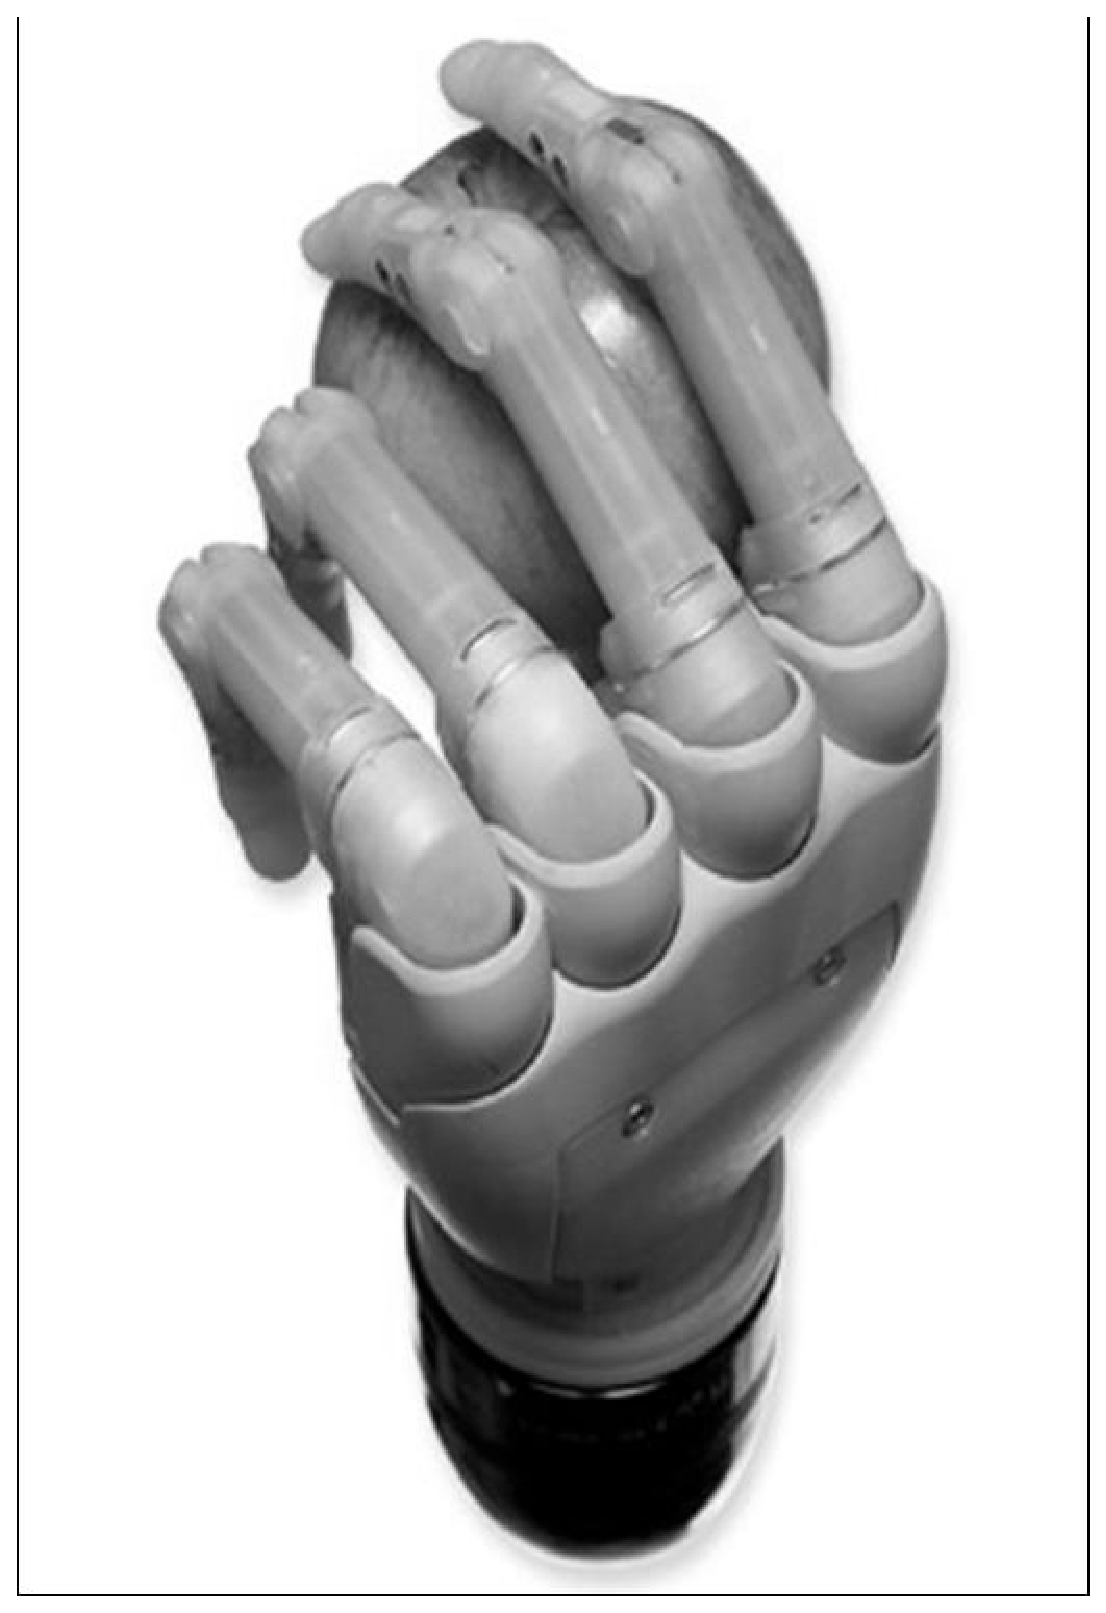
\includegraphics[width=0.25\textwidth]{hands_TB.eps} &
%%    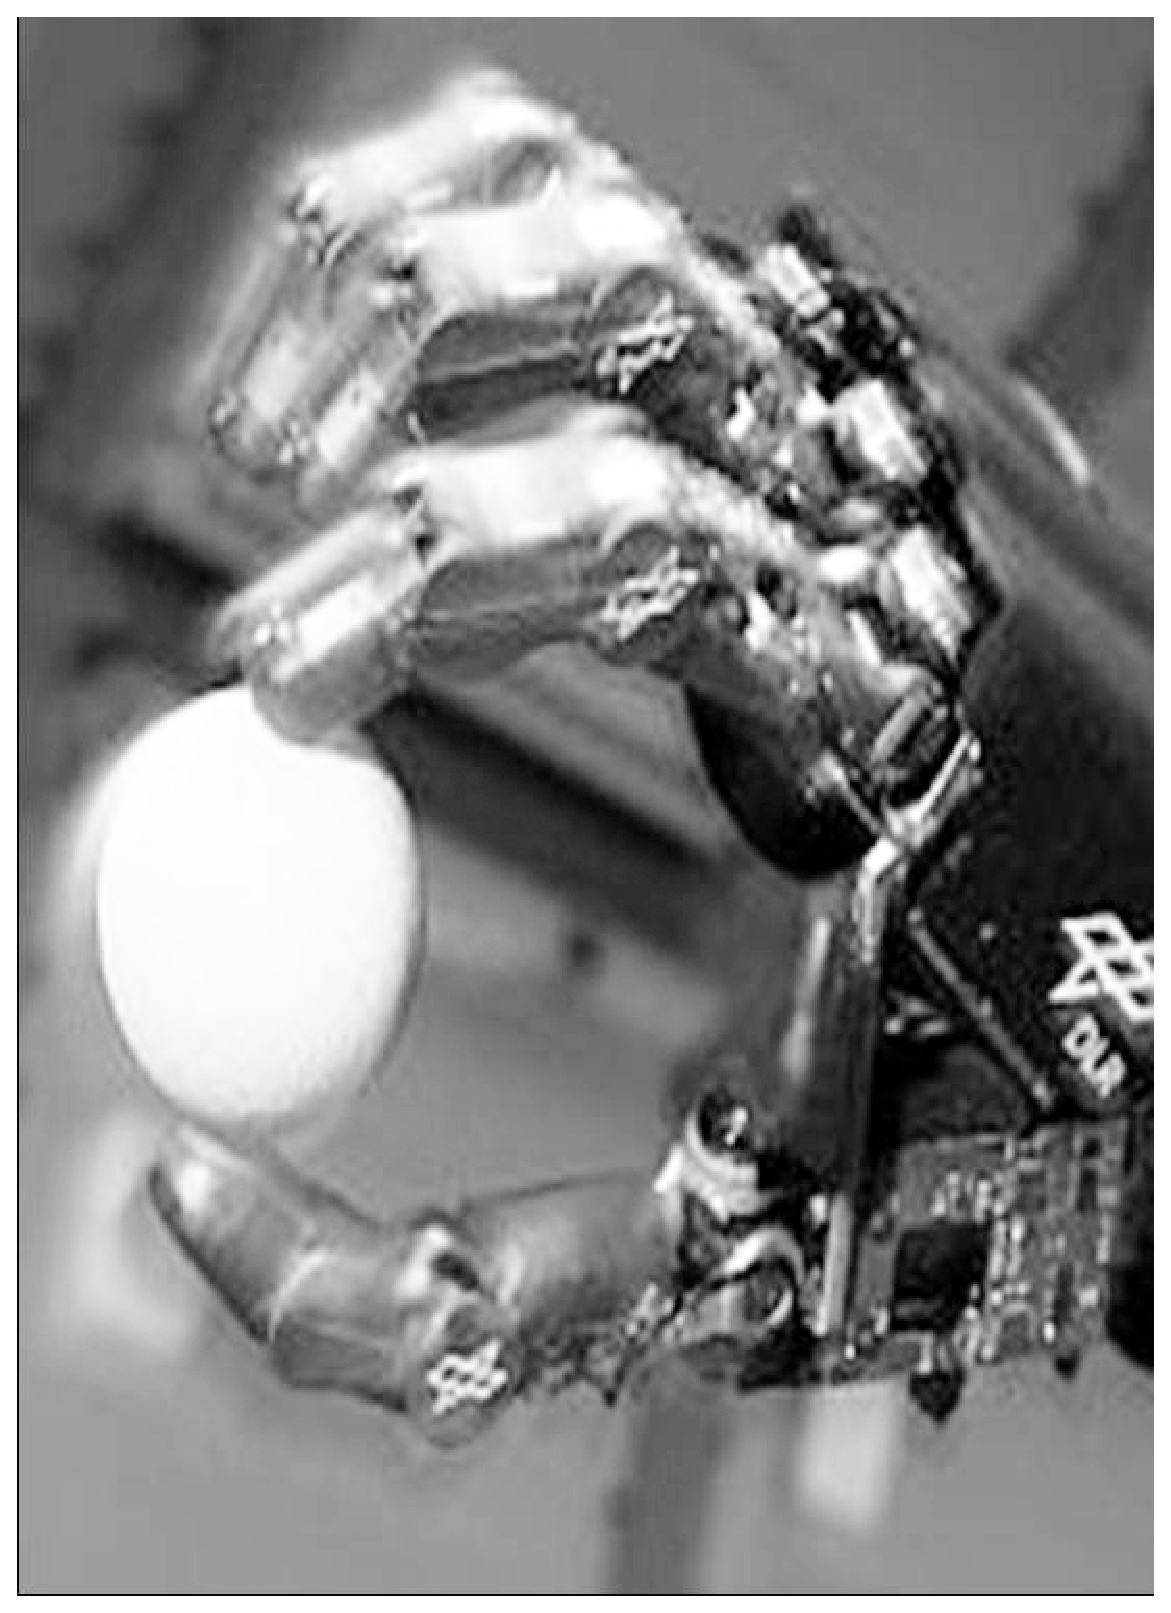
\includegraphics[width=0.25\textwidth]{hands_DLRII.eps} &
%%    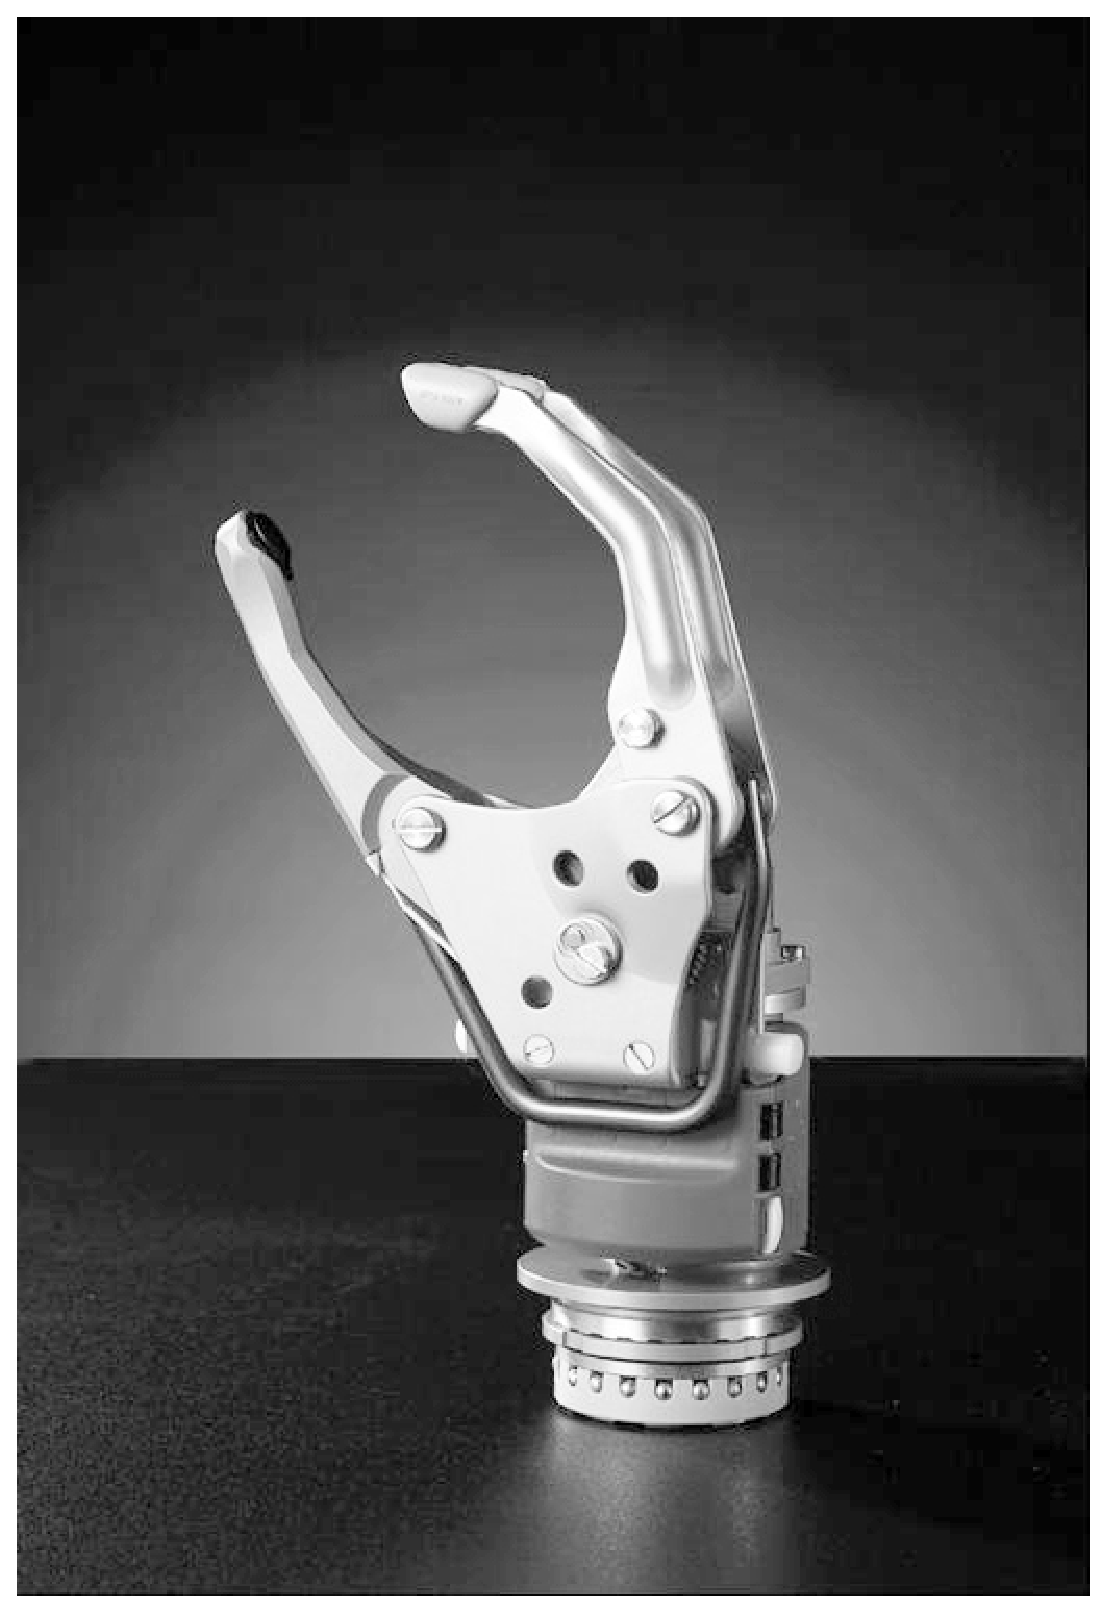
\includegraphics[width=0.25\textwidth]{hands_OB.eps} \\
%%    $(a)$ & $(b)$ & $(c)$
%%  \end{tabular}
%%  \end{center}
%  \caption{$(a)$ Touch Bionics's i-LIMB prosthetic hand (reproduced
%    from \cite{ilimb}); $(b)$ the DLR-II mechanical hand; $(c)$ Otto
%    Bock's SensorHand Speed (reproduced from \cite{sensorhand}).}
%  \label{fig:hands}
%\end{figure}

\begin{figure}[!t] \centering
%  \begin{tabular}{ccc}
%    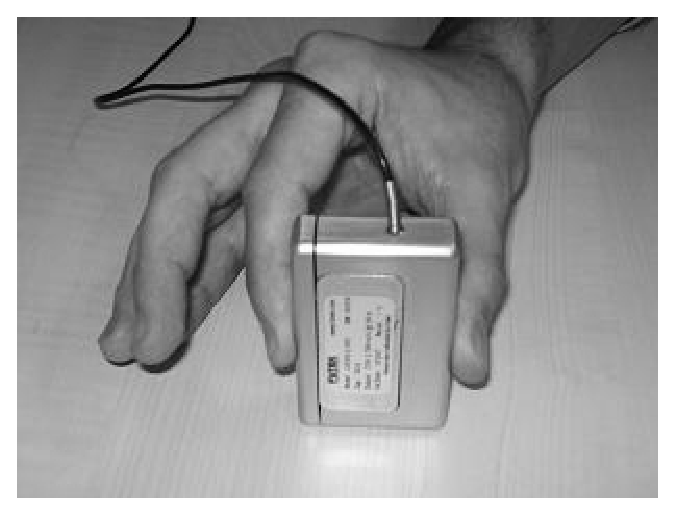
\includegraphics[height=0.16\textheight]{grip1.eps} &
%    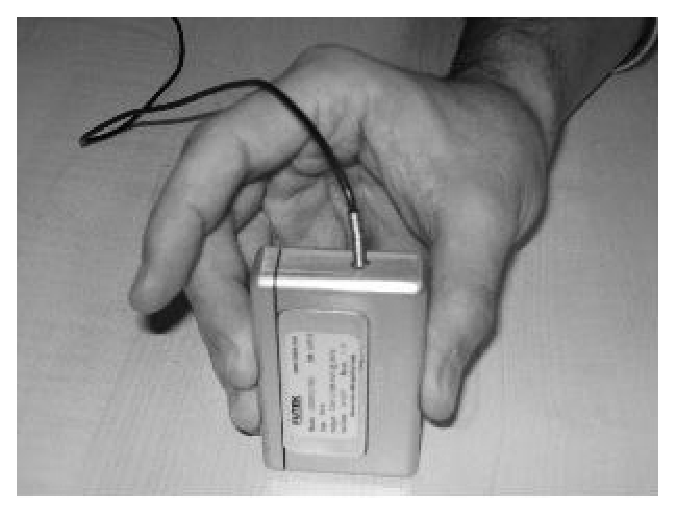
\includegraphics[height=0.16\textheight]{grip2.eps} &
%    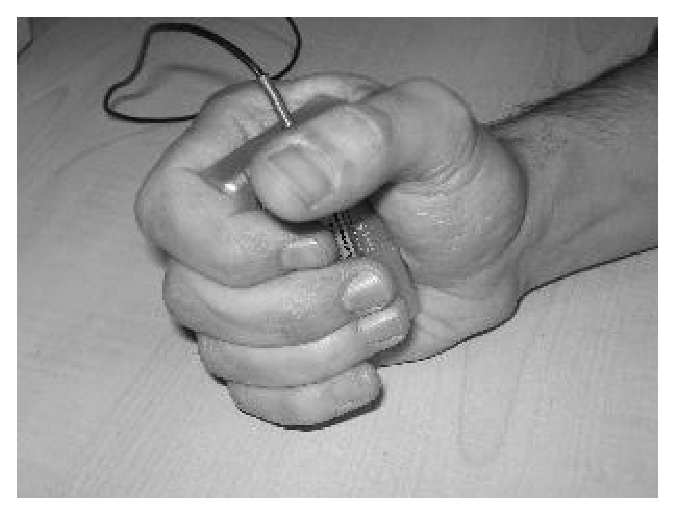
\includegraphics[height=0.16\textheight]{grip3.eps} \\
%    $(a)$ & $(b)$ & $(c)$ \\
%  \end{tabular}
  \caption{The three different grips employed in the experiment: $(a)$
   index precision grip; $(b)$ other fingers precision grip; $(c)$
   power grasp.}
  \label{fig:Grasps}
\end{figure}

\begin{figure}[!ht] \centering
%  \begin{tabular}{ccc}
%    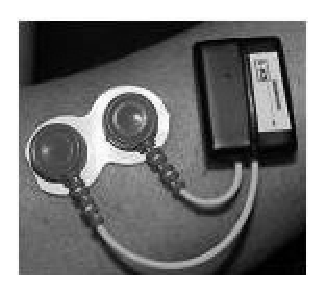
\includegraphics[height=0.16\textheight]{Electrode.eps} &
%    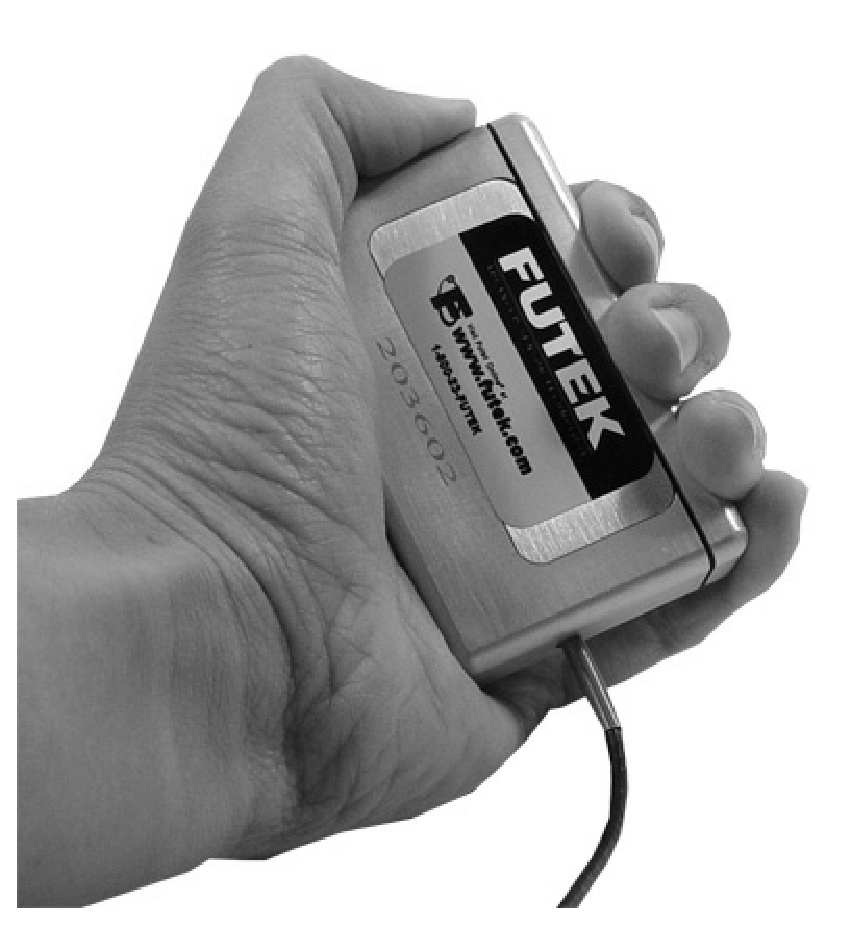
\includegraphics[height=0.16\textheight]{Hand_Gripper.eps} &
%    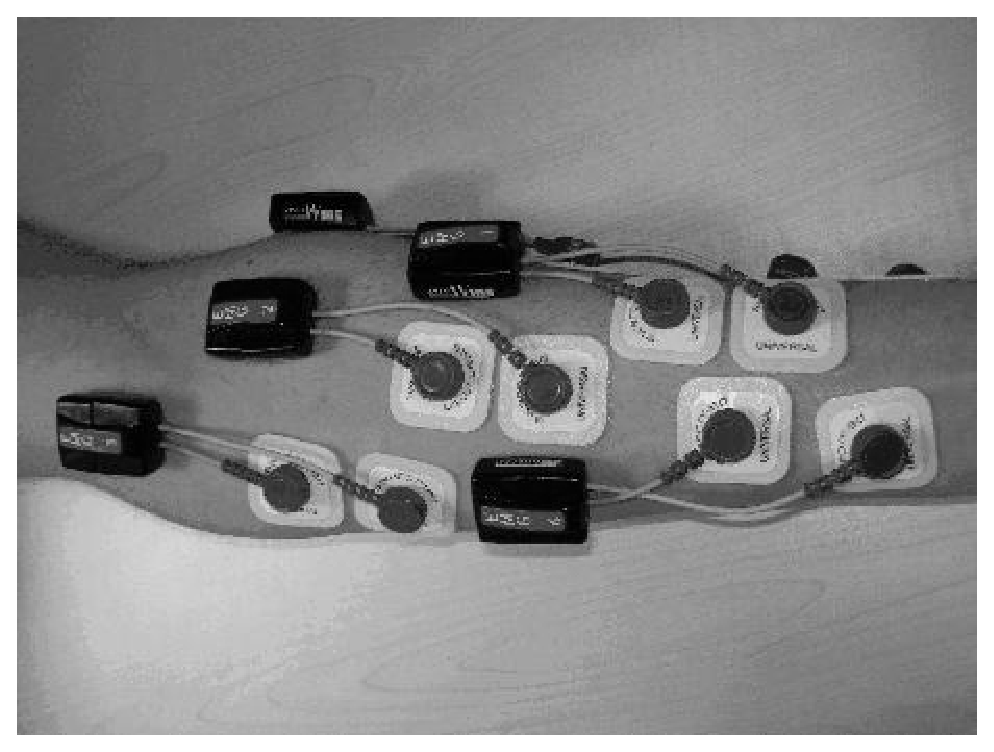
\includegraphics[height=0.16\textheight]{El_Arrangement.eps} \\
%    $(a)$ & $(b)$
%  \end{tabular}
  \caption{The experimental setup (\textit{subject side}): $(a)$ an EMG
    wireless electrode; $(b)$ the force sensor; $(c)$ typical
    placement of the EMG electrodes on a subject's forearm (ventral side).}
  \label{fig:SubjSetup}
\end{figure}

%\begin{figure}[!ht] \centering
%%  \begin{tabular}{cc}
%%    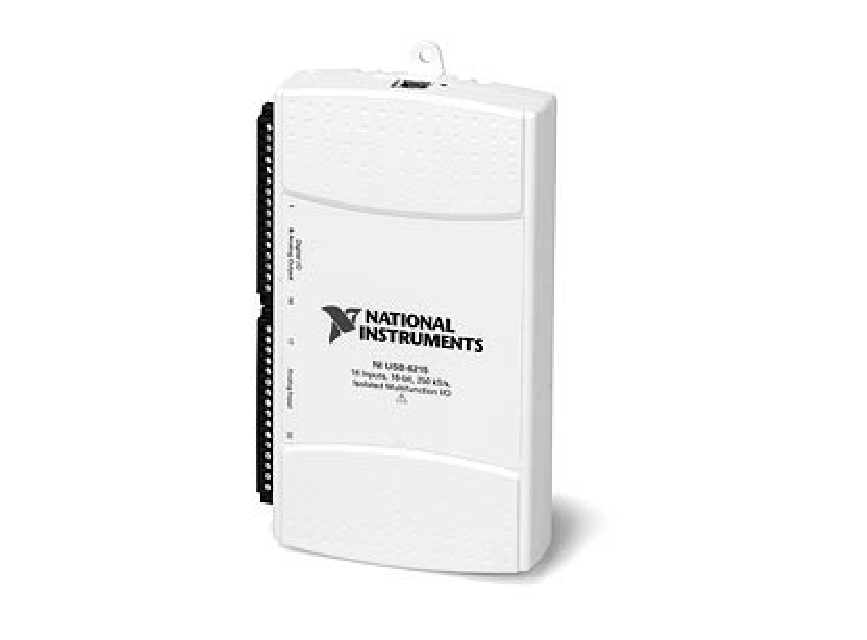
\includegraphics[height=0.16\textheight]{NI-6211.eps} &
%%    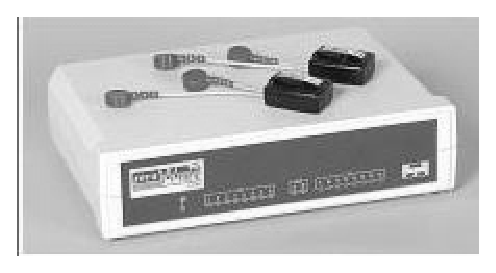
\includegraphics[height=0.16\textheight]{Zero_Base.eps} \\
%%  $(a)$ & $(b)$\\
%%  \end{tabular}
%  \caption{The experimental setup (\textit{experimenter side}): $(a)$
%   the USB data acquisition card (NI-USB6211); $(b)$ the EMG device
%   receiver.}
%  \label{fig:ExpSetup}
%\end{figure}

\begin{figure}[!ht] \centering
%  \begin{tabular}{cc}
%    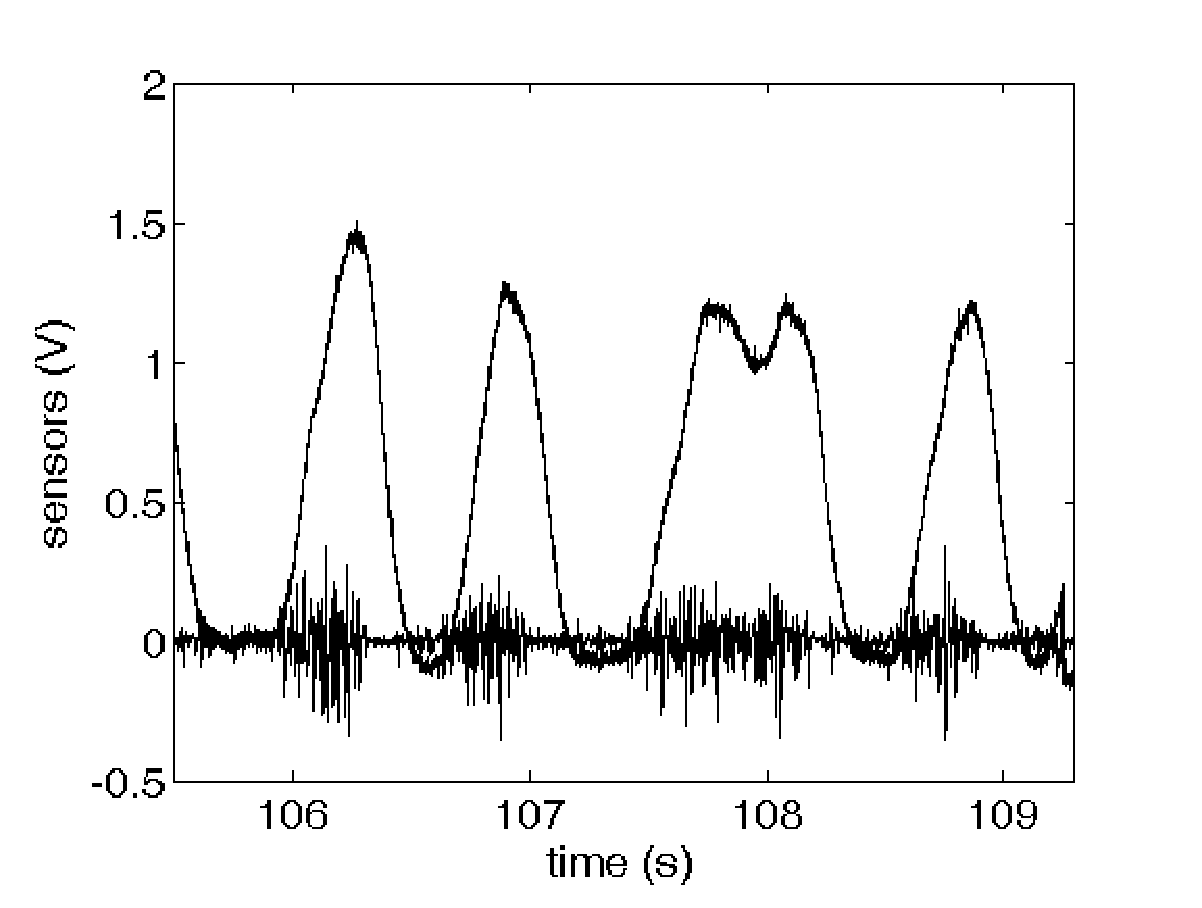
\includegraphics[width=0.45\textwidth]{force_raw.eps} &
%    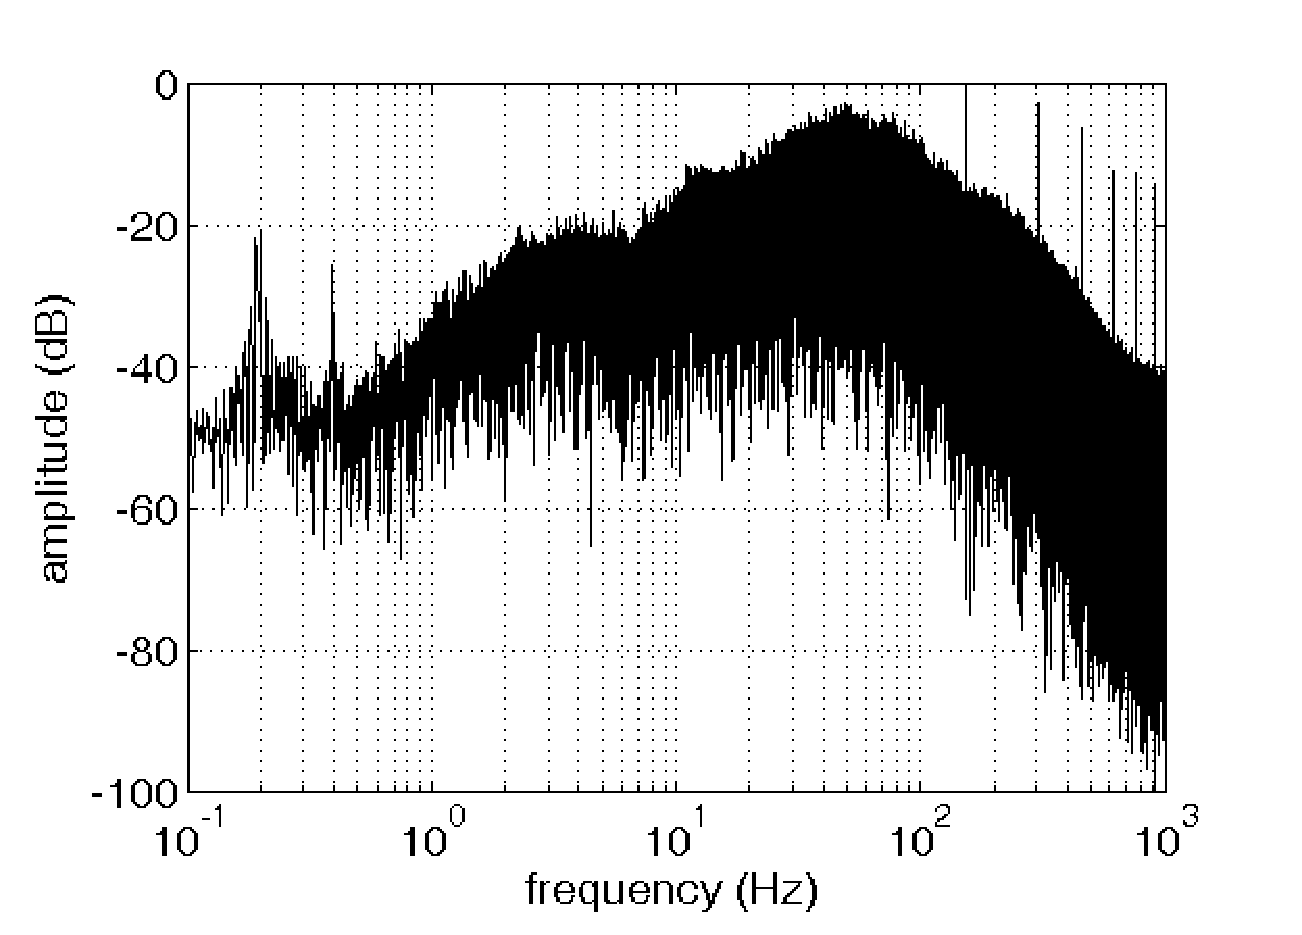
\includegraphics[width=0.45\textwidth]{spectrum_raw.eps} \\
%    $(a)$ & $(b)$ \\
%  \end{tabular}
  \caption{$(a)$ typical raw EMG (red) and force (blue) signals, as read from the
    electrodes and force sensor; $(b)$ frequency diagram of the EMG signal.}
  \label{fig:spectra}
\end{figure}

\begin{figure}[!ht] \centering
%  \begin{tabular}{ccc}
%    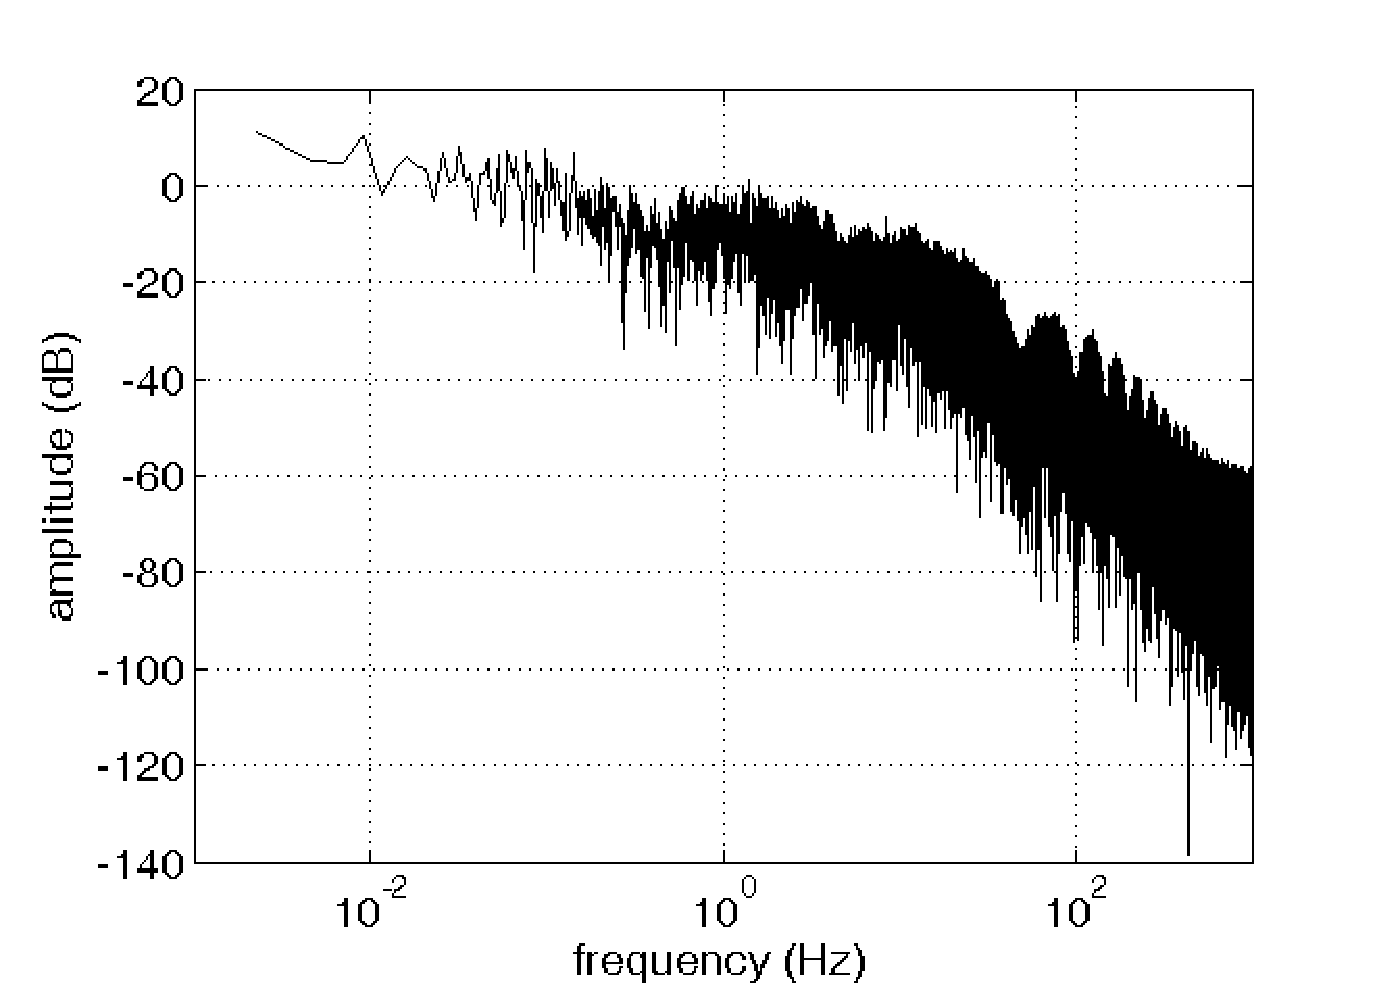
\includegraphics[width=0.3\textwidth]{spectrum_RMS0040.eps} &
%    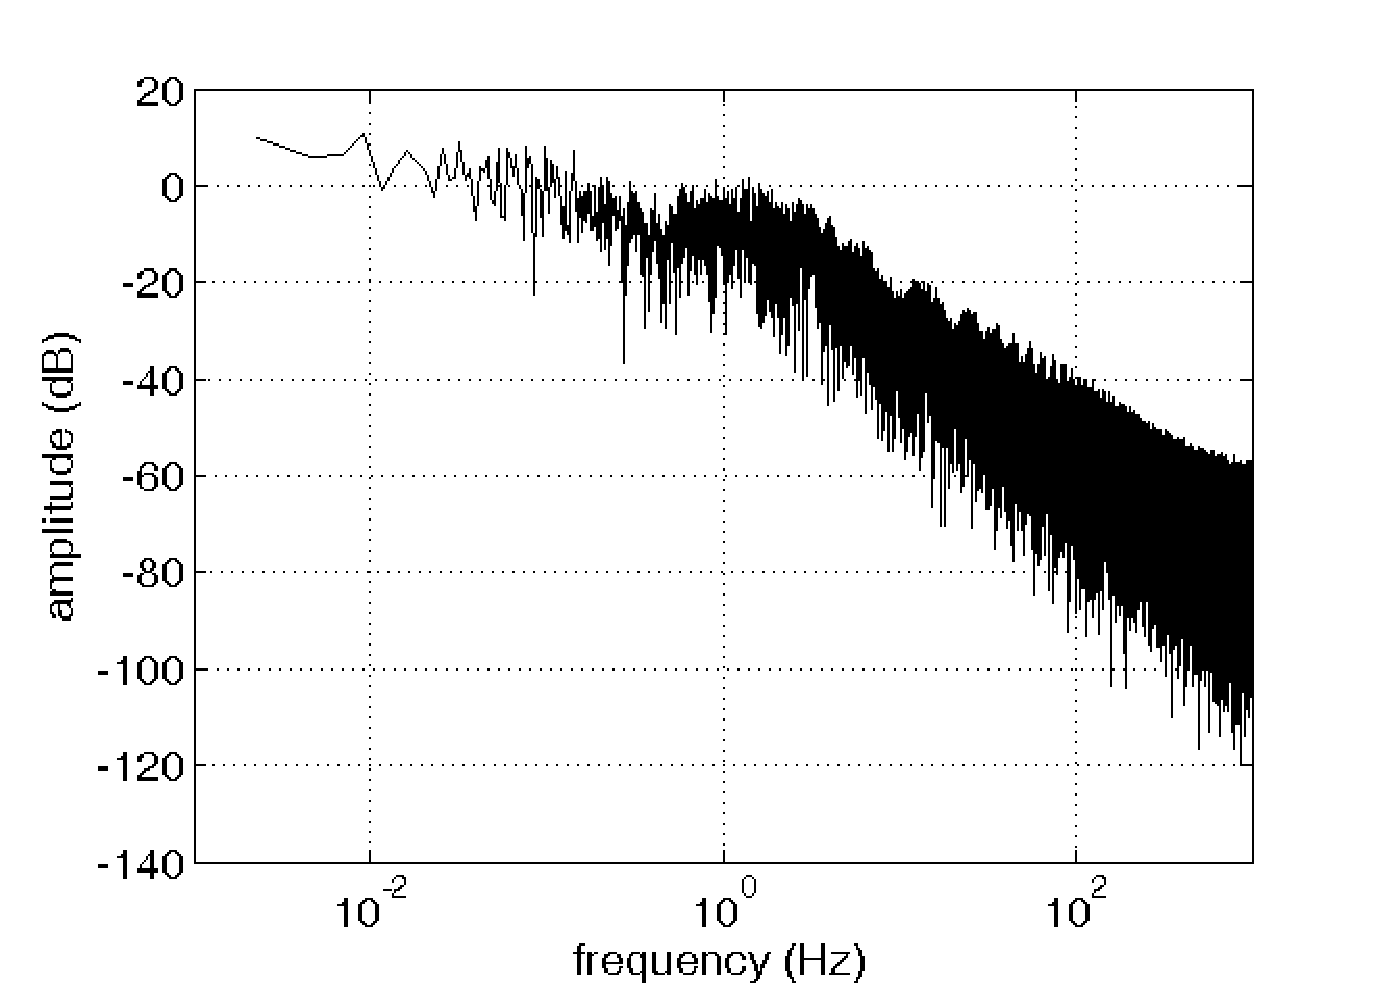
\includegraphics[width=0.3\textwidth]{spectrum_RMS0200.eps} &
%    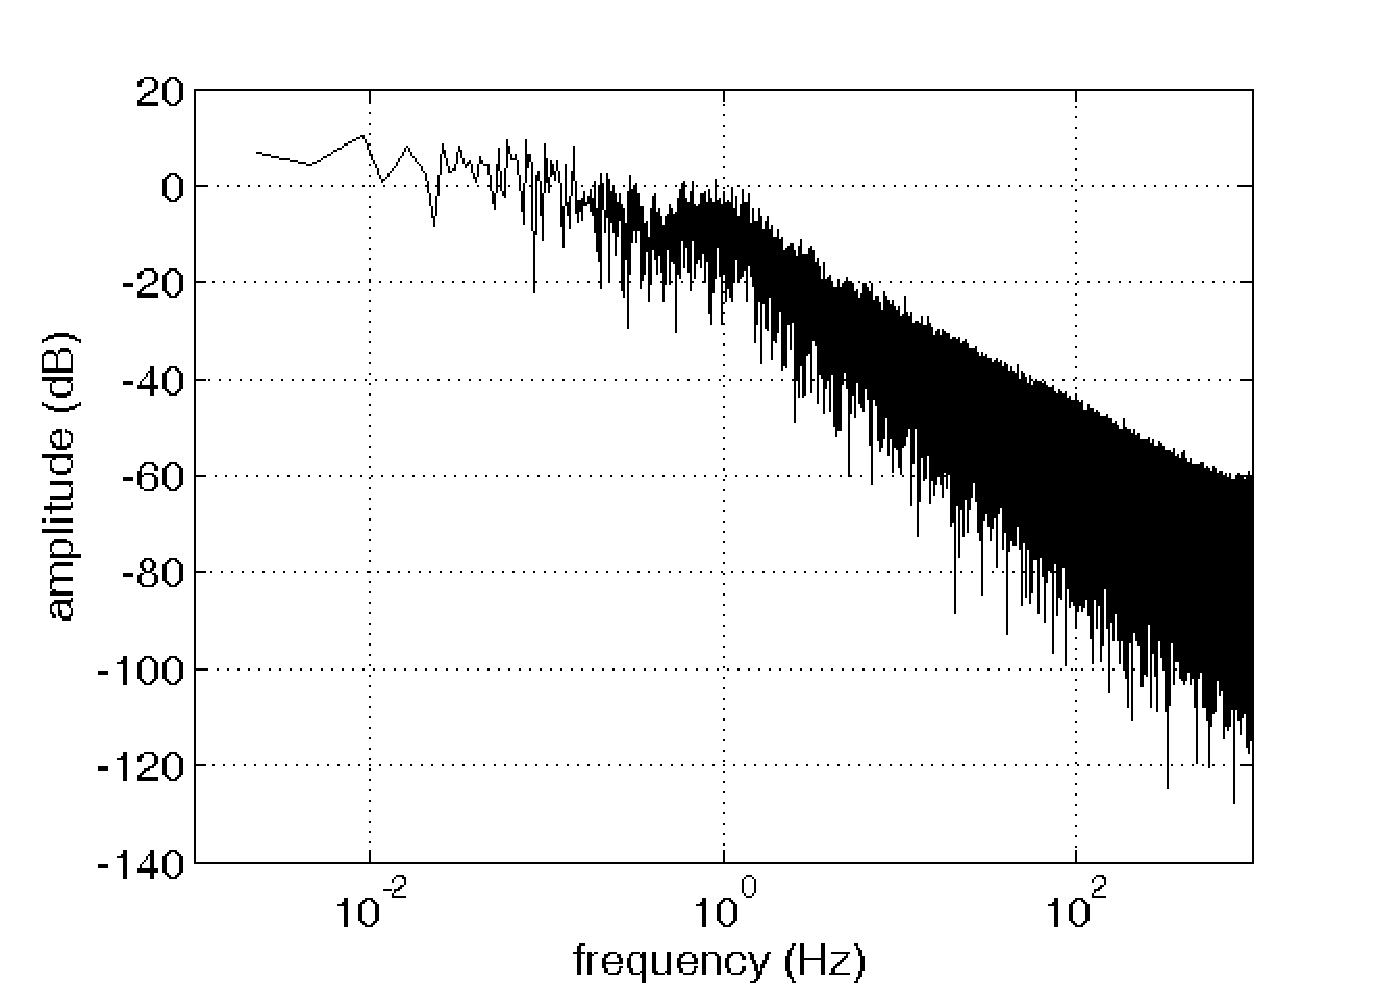
\includegraphics[width=0.3\textwidth]{spectrum_RMS1000.eps} \\
%    $(a)$ & $(b)$ & $(c)$ \\
%  \end{tabular}
  \caption{(left to right) effects of the RMS on the bandwidth of the EMG
    signals, for $T_{RMS} = 20, 100, 500ms$.}
  \label{fig:RMSs}
\end{figure}

%\begin{figure}[!ht] \centering
%%  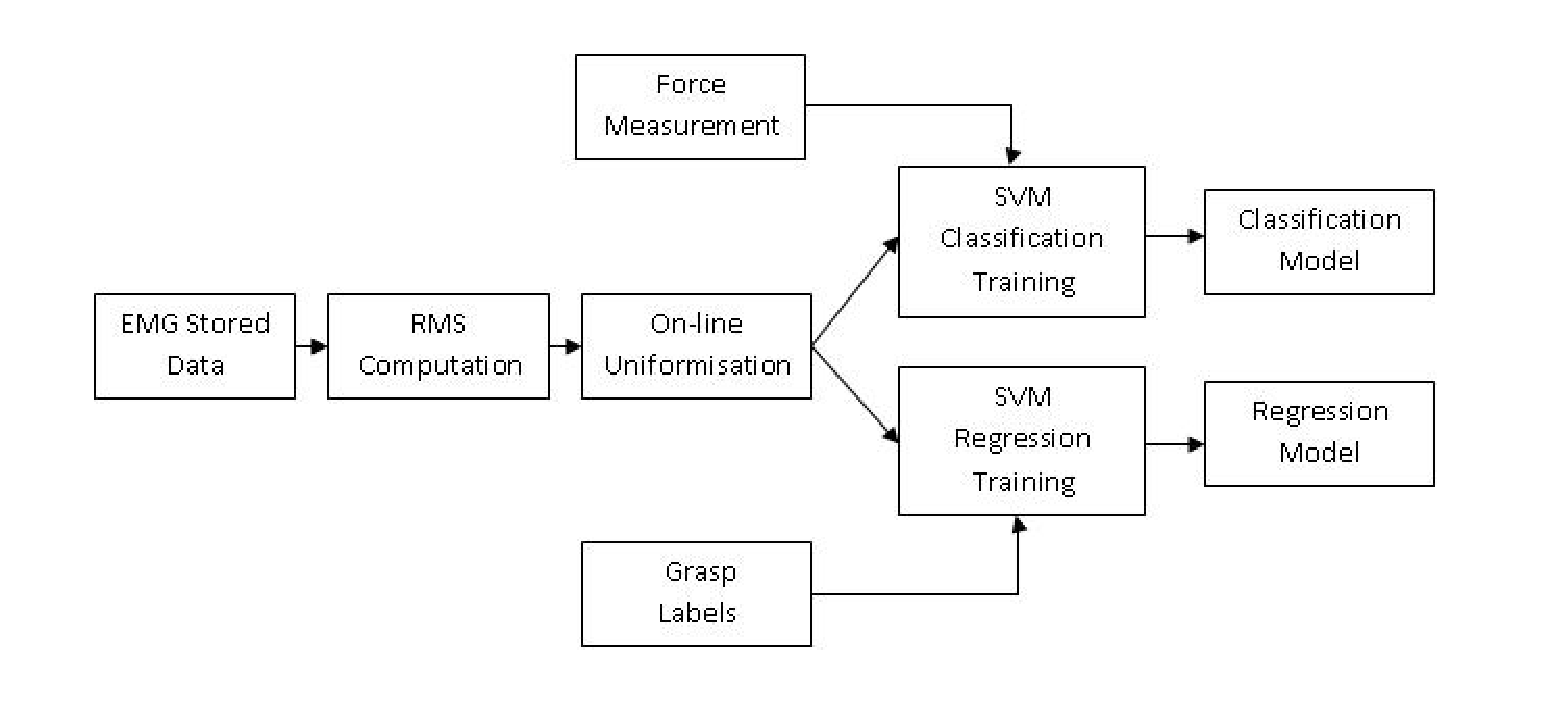
\includegraphics[width=0.75\textwidth]{Schema.eps} \\
%  \caption{Graphical representation of the system employed to solve our problem.}
%  \label{fig:Algorithm}
%\end{figure}

\begin{figure}[!ht] \centering
%  \begin{tabular}{cc}
%    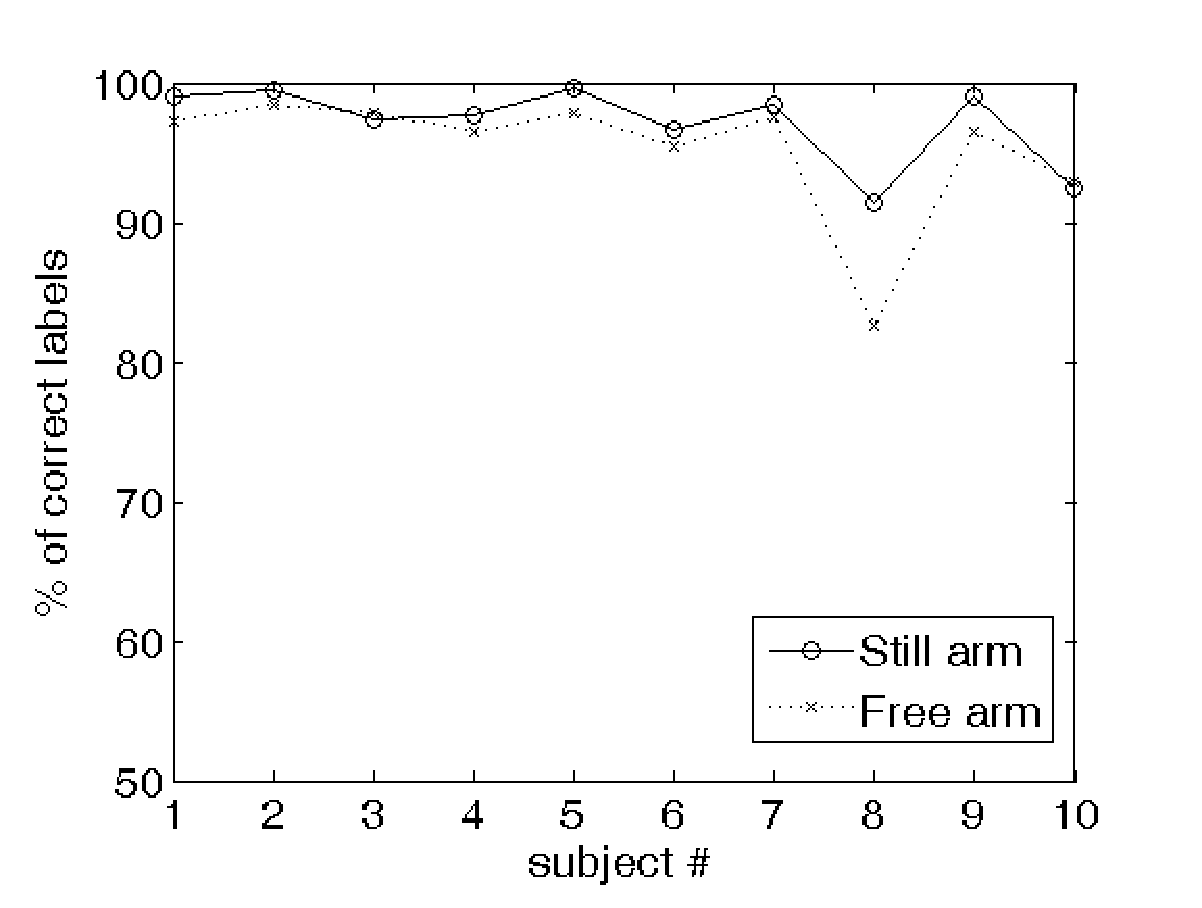
\includegraphics[width=0.45\textwidth]{perfClass.eps} &
%    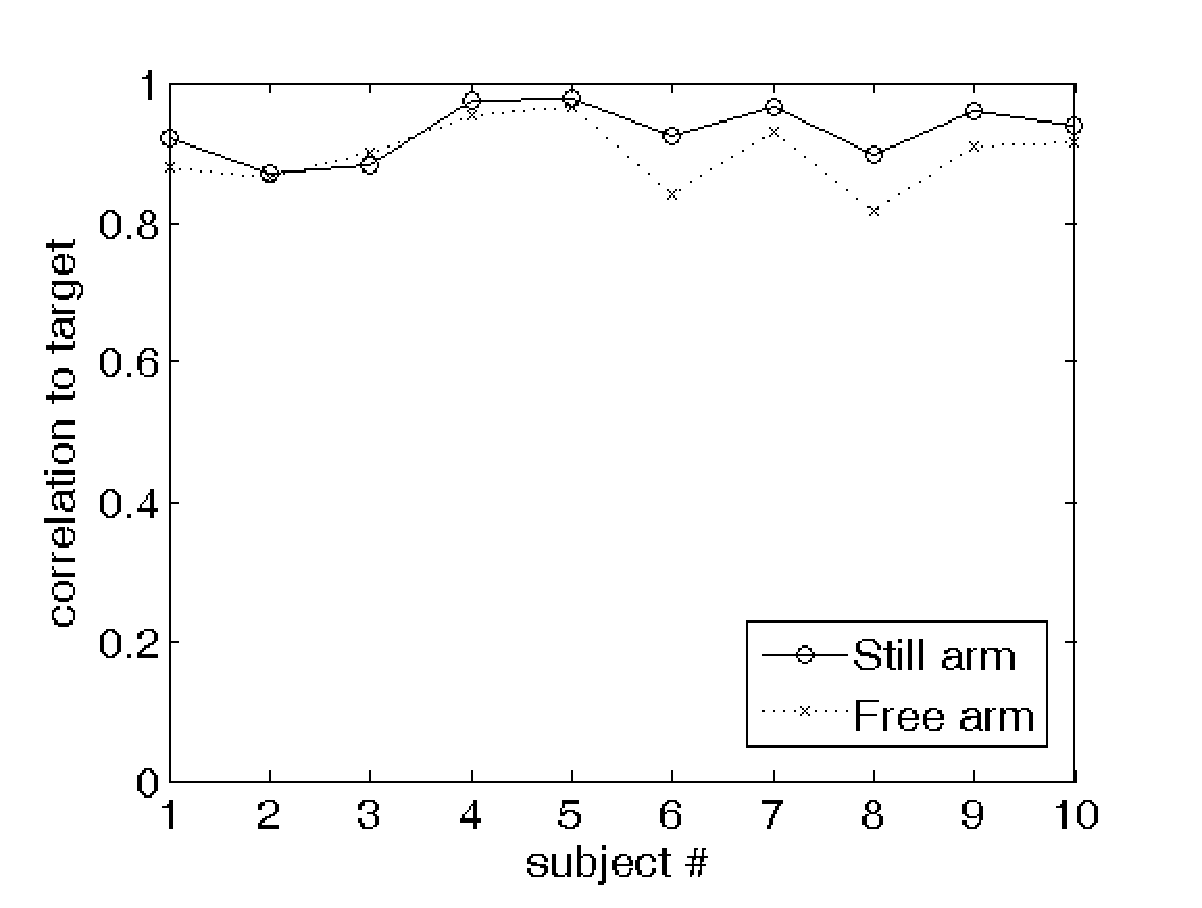
\includegraphics[width=0.45\textwidth]{perfRegr.eps} \\
%    $(a)$ & $(b)$ \\
%  \end{tabular}
  \caption{classification (top) and regression (middle, correlation to target;
    bottom, NRMSE) results obtained by the system, on both phases of the
    experiment (FA and SA) and for each subject.}
  \label{fig:results}
\end{figure}

\begin{figure}[!ht] \centering
%  \begin{tabular}{cc}
%    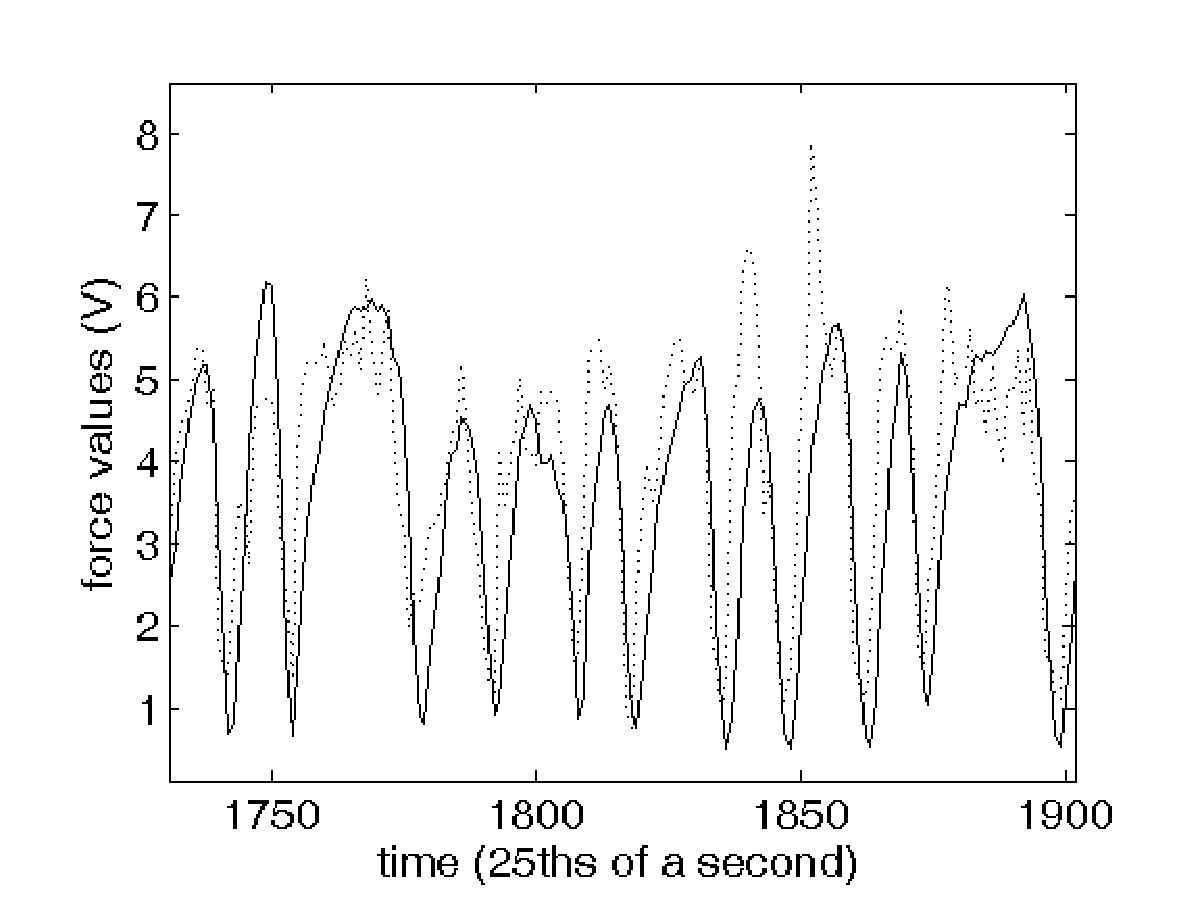
\includegraphics[width=0.45\textwidth]{example_6_one.eps} &
%    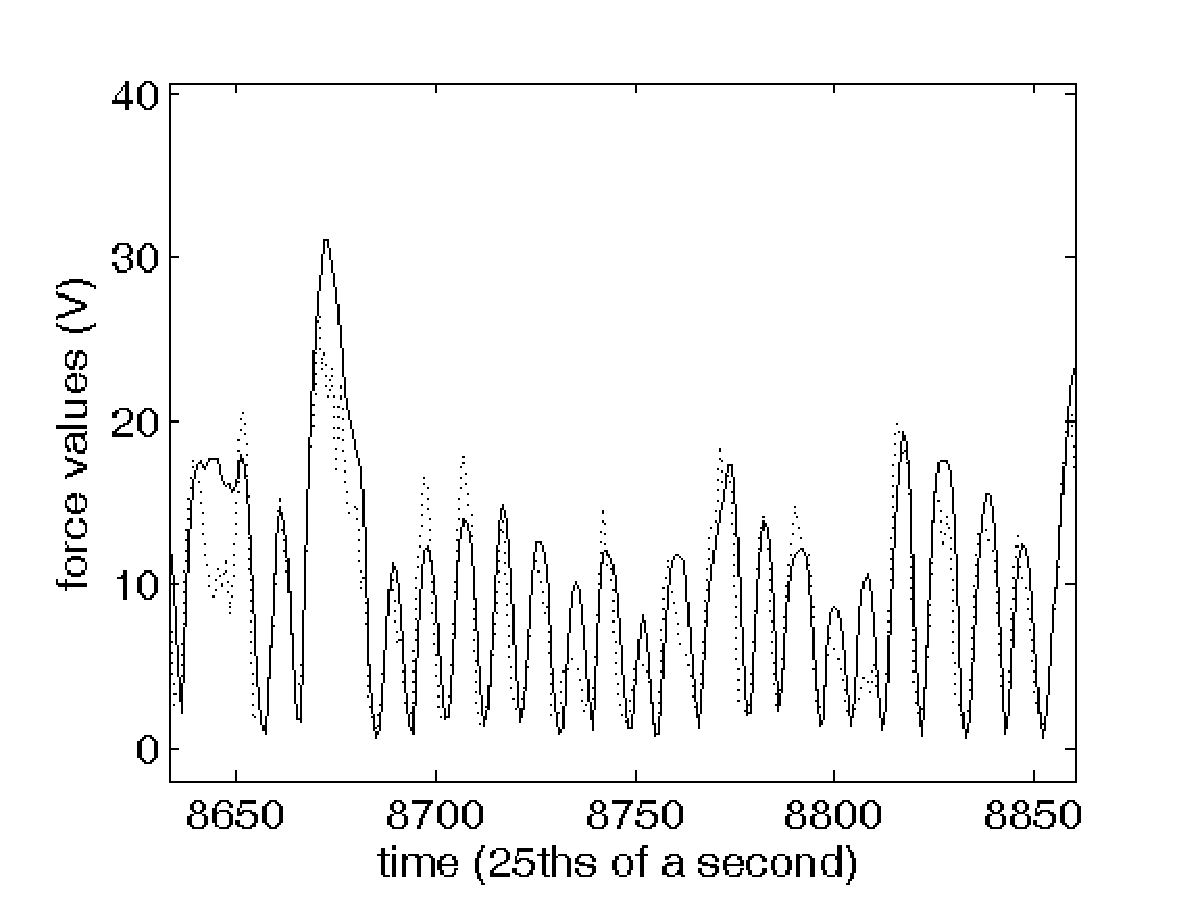
\includegraphics[width=0.45\textwidth]{example_6_two.eps} \\
%    $(a)$ & $(b)$ \\
%  \end{tabular}
  \caption{comparing true (continuous line) and guessed (dotted line) force values for regression of a
    typical subject (number $6$, FA phase).}
  \label{fig:examples}
\end{figure}

\begin{figure*}[!ht] \centering
%  \begin{tabular}{cc}
%    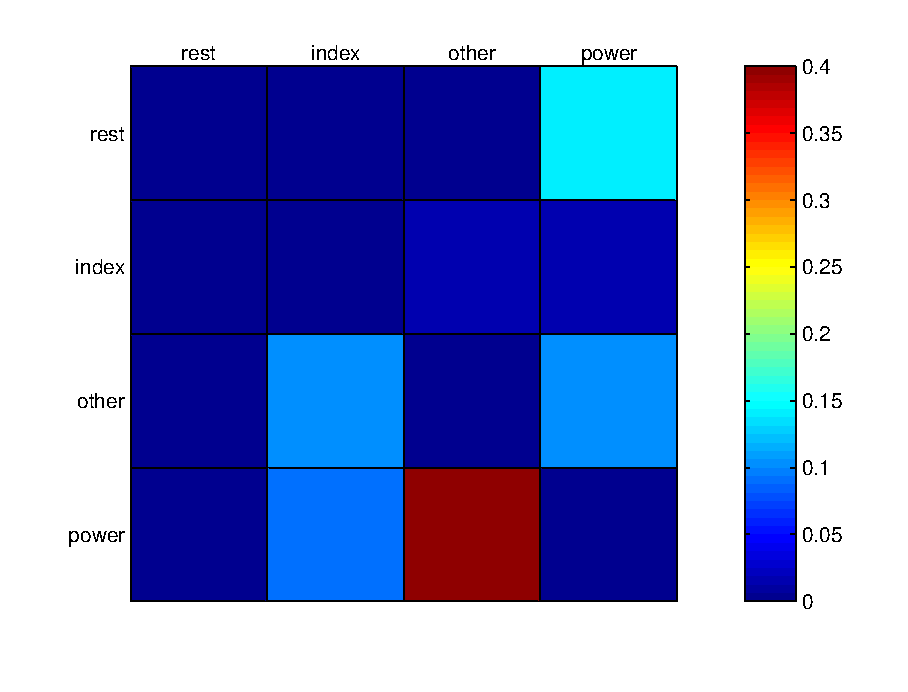
\includegraphics[width=0.45\textwidth]{confMat_1.eps} &
%    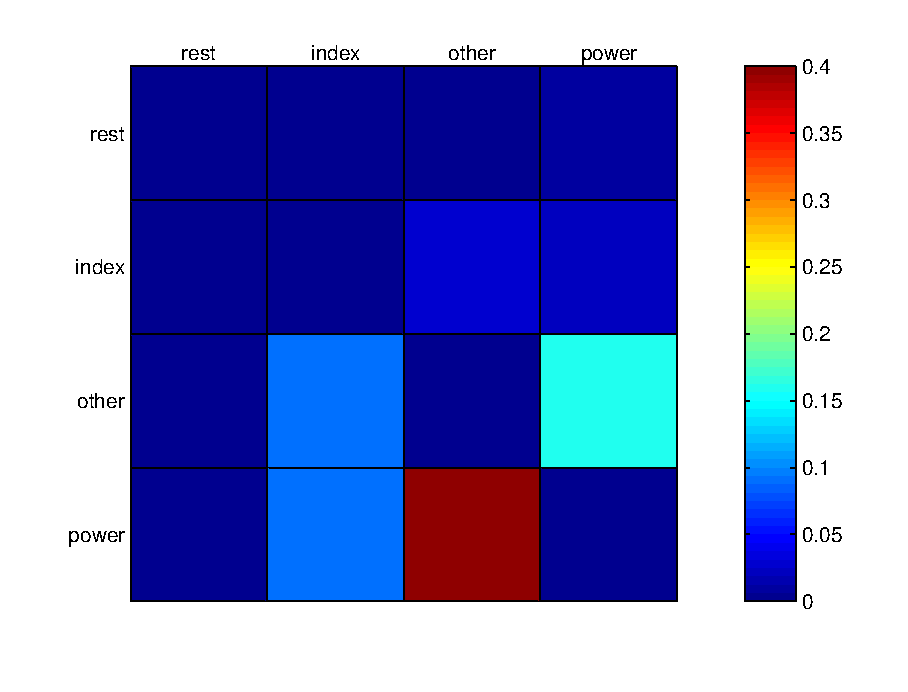
\includegraphics[width=0.45\textwidth]{confMat_2.eps} \\
%  \end{tabular}
  \caption{confusion matrices for the SA phase (left) and FA phase (right). Each matrix
           is the average over the confusion matrices of the $10$ subjects. A confusion
           matrix $C$ is such that its $(i,j)$th element is the fraction of $i$ labels
           mistaken for $j$ labels, over the total mistaken labels.}
  \label{fig:confusion}
\end{figure*}

\begin{figure}[!ht] \centering
%  \begin{tabular}{cc}
%    \includegraphics[width=0.45\textwidth]{2on1_class.eps} &
%    \includegraphics[width=0.45\textwidth]{2on1_regr.eps} \\
%    $(a)$ & $(b)$ \\
%  \end{tabular}
   \caption{classification (top) and regression (bottom, correlation to target)
      results obtained testing on SA-data models trained on FA, and vice-versa.}
  \label{fig:2on1}
\end{figure}

\begin{figure}[!ht] \centering
%  \begin{tabular}{c}
%    \includegraphics[width=0.6\textwidth]{subj8.eps} \\
%  \end{tabular}
  \caption{size of the training set (dotted line) and classification
    performance (continuous line), of subject $8$ in the FA phase, as
    $d$ changes.}
  \label{fig:subj8}
\end{figure}

\begin{figure}[!ht] \centering
%  \begin{tabular}{cc}
%    \includegraphics[width=0.45\textwidth]{crossClass1.eps} & \includegraphics[width=0.45\textwidth]{crossClass2.eps} \\
%    $51.69\% \pm 19.27\%$ & $54.04\% \pm 16.42\%$ \\
%    \includegraphics[width=0.45\textwidth]{crossRegr1.eps} & \includegraphics[width=0.45\textwidth]{crossRegr2.eps} \\
%    $0.60 \pm 0.18$ & $0.58 \pm 0.19$ \\
%  \end{tabular}
  \caption{cross-subject performance matrices, for classification (top
    row) and regression (bottom row), in the SA (left column)
    and FA phase (right column); the numbers refer to all element of
    the matrices, excluding the diagonals.}
  \label{fig:cross}
\end{figure}

\end{bmcformat}

\end{document}
